\documentclass[a4paper,12pt]{article}

%% Standard
\usepackage[ngerman]{babel} 
\usepackage[utf8]{inputenc}
\usepackage[T1]{fontenc}

%% Mathe
\usepackage{amsmath}
\usepackage{amssymb}
\usepackage{amsthm}
\usepackage{latexsym}

%% Aufzaehlungen
\usepackage{enumerate}

%% Bilder
\usepackage{subfigure}
\usepackage{graphicx}
\usepackage{wrapfig}

%% Absaetze usw
\usepackage{multicol}   
% zu verwenden mit 
% \begin{multicols}{$$Spaltenanzahl$$} 
%  text...
% \end{multicols}

%\setlength{\parindent}{0pt}    %Absatz-Einrueckung
%\setlength{\parskip}{3pt}      %Absatz-Abstaende


%% Fusszeilen
\usepackage{fancyhdr}
\pagestyle{fancy}
\renewcommand{\headrulewidth}{0pt}
\renewcommand{\footrulewidth}{0.4pt}
\lfoot{\NAME : \TITEL}
\cfoot{}
\rfoot{\thepage}
\lhead{}
\chead{}
\rhead{}
%\setlength{\headheight}{15pt}


%% Links
\usepackage[colorlinks=true,linkcolor=black,citecolor=black,%
bookmarksnumbered=true,breaklinks=true,pdfstartview=FitH]{hyperref}

%% Eigene Kommandos
% Differenzialrechnung
\newcommand{\diff}{\ensuremath{\mathrm d}}
\newcommand{\dx}{\ensuremath{\mathrm dx}}
\newcommand{\dvx}{\ensuremath{\mathrm d \vec x}}

% Lineares
\newcommand{\Mat}[1]{\ensuremath{\mathbf{#1}}}
\newcommand{\Ten}[1]{\ensuremath{\mathcal{#1}}}
\newcommand{\Ve}[1]{\ensuremath{\vec{#1}}}
% Vektoren sind Fette buchstaben
\renewcommand{\vec}[1]{\ensuremath{\boldsymbol{#1}}}
% Vektoren sind fett und nicht kursiv
% \renewcommand{\vec}[1]{\ensuremath{\mathbf{#1}}}
\newcommand{\skp}[2]{\ensuremath{\langle #1 \,|\, #2 \, \rangle}}


% Euler
\newcommand{\e}{\ensuremath{\operatorname{e}}}
\newcommand{\E}{\ensuremath{\operatorname{e}}}
\newcommand{\ir}{\ensuremath{\operatorname{i}}}
\newcommand{\I}{\ensuremath{\operatorname{i}}}

% allg Mathe
\newcommand{\R}{\ensuremath{\mathbb{R}}}
\newcommand{\folgt}{\ensuremath{\Rightarrow}}
\newcommand{\gdw}{\ensuremath{\Leftrightarrow}}


% Formatierung
\newcommand{\abs}[0]{\bigskip\noindent}
\newcommand{\const}{\ensuremath{\text{\emph{const}}}}
\newcommand{\fixme}[0]{{\bf \Huge FIXME}}
\newcommand{\inh}[1]{{\bf #1}}


% Umgebungen
\newtheorem{satz}{Satz}[section]
\newtheorem{defi}{Definition}[section]
\newtheorem{lemma}{Lemma}[section]





%% Captions %%
% FOrmatiert die Captions bei Bildern um
% \usepackage[%
% %singlelinecheck=false,%einzeiler werden nicht zentriert.
% %font={%Schriftformatierung
% labelfont={%Formatierung von ``Abbildung''
% bf,it%fett und kursiv
% },%
% textfont={%Formatierung von Text
% %small,%kleinere schrift
% %it%kursiv
% sl
% },%
% ]{caption}
\usepackage[labelfont={bf,it},textfont={sl}]{caption}





\begin{document}



\newcommand{\NAME}{Michael Springer \& Kopp }
\newcommand{\FACH}{Fortgeschrittenenpraktikum}
\newcommand{\TITEL}{ESR}
\newcommand{\DATUM}{\today}


\pagestyle{plain} 
	% auskommentieren fuer fusszeile



%%%% Eigener Kopf

\sloppy

\begin{center}
\FACH
\hfill
\DATUM
\end{center}

\vspace{-5mm} % weniger abstand

\begin{center}
  \begin{Large}
 \textbf{\TITEL}
  \end{Large}
\end{center}

\vspace{-3mm}

\begin{center}
\hrulefill
%\quad
 %\raisebox{-1.5mm}{\NAME}
% \,
\quad 
\textit{\NAME}
\,
\hrulefill
\end{center}
 
 
%%%%%%%%%%%%%%%%%%%%%%%%%%%%%
%%%%%%%%%%%%%%%%%%%%%%%%%%%%%%
%%%%%%%%%%%%%%%%%%%%%%%%%%%%%%%%








\section{Einleitung}

Bei der Elektronenspinresonanz -- kurz ESR -- handelt es sich um ein
spektroskopisches Verfahren, in dem man das Verhalten von ungepaarten
Elektronen in einem externen Magnetfeld untersucht.

Weil hier f"ur die eigentliche Spektroskopie Mikrowellen verwendet
werden, wird sich der erste Teil des Versuchs mit der Erzeugung,
Leitung, allgemeinen Charakteristika etc. von Mikrowellen befassen.

Im zweiten Teil werden wir dann die ESR-Versuche wirklich
durchf"uhren. Dazu untersuchen wir Eigenschaften des Aufbaus und
optimieren bzw. eichen die Anlage f"ur Messungen und untersuchen den
Einfluss verschiedener Parameter auf die Messwerte.

"Uber die aufgenommen Spektroskopiekurven bestimmen wir den $g$-Faktor
von Mangan-II-Ionen, die Hyperfeinstrukturkonstante von
Mangan-II-Ionen und
TEMPO\footnote{(2,2,6,6-Tetramethyl-1-Piperidin-1-Oxyl) in Toluol
  gel"ost}, aus"serdem Komponenten des $g$-Tensors von
Kupfer-II-Ionen.

Indem wir die Linienformen von DPPH und Mn-II genauer untersuchen,
k"onnen wir dar"uber hinaus den Kernspin von Stickstoff-14 und
Mangan-55 bestimmen und jeweils die Aufenthaltswahrscheinlichkeit der
ungepaarten Elektronen am Ort des Kerns berechnen.

Im letzten Teil des Versuchs konnten wir dar"uber hinaus noch einen
weiteren Quantenmechanischen Effekt beobachten: Den Spin-Austausch und
die damit verbundene Lebendsdauer der Zust"ande.




\clearpage
\tableofcontents
\clearpage


\section{Theoretische Grundlagen: Mikrowellen}
\label{sec:theor_grundl_mikr}


\subsection{Erzeugung von Mikrowellen im Klystron}
\label{sec:erze_von_mikr_im_klystr}


Ein kontinuierlicher Elektronenstrom wird aus einer Kathode
abgegeben. Die Elektronen durchqueren einen Hohlraumresonator mit zwei
Gittern, die von den Elektronen passiert werden. In dem
Hohlraumresonator ist eine stehende (elektromagnetische) Welle. Das
oszillierende Elektrische Feld derselben wirkt auf den
Elektronenstrom. Hier werden Elektronen abgebremst oder Beschleunigt,
je nachdem wie das E-Feld gerade orientiert ist (bei stehenden
elektromagnetischen Welle oszilliert das E-Feld). Als Effekt davon
bilden die Elektronen nunmehr kleien Gr"uppchen --
d.h. "`Verdickungen"' und "`Verd"unnungen"' im Elektronenstrom hinter
dem Resonator.

Haben die Elektronen die beiden Gitter einmalig durchquert, treffen
sie auf einen Reflektor. Dort werden sie zur"uckgeworfen und nehmen
den Weg zur"uck zum Hohlraumresonator. Die Spannung am Reflektor
("`Reflektorspannung"') kann von uns moduliert werden.

Die Reflektorspannung muss nun so gew"ahlt werden, dass die
Elektronen, die zur"uckkommen, beim Durchqueren des Gitters ein E-Feld
darstellen, das gerade in Phase mit dem E-Feld der stehenden EM-Welle
im Resonator ist. Dann wird Energie aus dem Elektronenstrom gezogen
und das E-Feld -- und dmait die EM-Welle -- im Resonator
gest"arkt. Die Elektronen bilden das (oszillierende) E-Feld dadurch,
dass am Ort des Gitters die "ortliche "`Haufenbildung"' einer
zeitlichen "`Haufenbildung"' entspricht. Die verschiedenen
"`Verdickungen"' und "`Verd"unnungen"' gehen mit einer erh"ohten
bzw. verminderten Ladungsdichte -- und damit einem E-Feld einher.

Die Stehende Welle im Resonator wird schlie"slich als Mikrowelle
ausgekoppelt.

Die Mikrowellenfrequenz h"angt damit von der Abmessung des Resonators,
aber auch von der Frequenz der Reflektorspannung ab. Die Gr"o"se des
Resonators ist durch eine Stellschraube verstellbar, womit man das
Klystron bei gegebener Reflektorspannung genauer auf eine Frequenz
einstellen kann.


\subsection{Leitung im Hohlleiter}
\label{sec:leitung_im_hohlleiter}

Wir leiten die Mikrowellen in Hohlleitern. Hier ist um den
luftgef"ullten Bereich, in dem sich die Mikrowellen fortpflanzen
sollen eine metallene H"ulle mit rechteckigem Querschnitt.

Die metallene H"ulle ist ein Leiter und ein solcher stellt
Randbedingungen an die Elektromagnetische Welle dar: Das Elektrische
Feld darf nurnoch eine Normal- und das magnetische Feld eine
Parallelkomponente auf die jeweiligen Leiter haben.

Mit diesen Bedingungen folgt, dass im Hohlleiter nur bestimmte --
diskrete -- Wellen zugelassen sind. Diese unterscheiden sich dadurch,
wie viele B"auche bzw. Knoten die spezielle Welle in die beiden
Richtungen senkrecht zur Ausbreitungsrichtung hat.  Die
Randbedingungen diktieren nun, diese Anzahlen jeweils ganzzahlig sein
m"ussen.  Eine solche, durch zwei Ganzzahlen charakterisierte Welle
bezeichnet man als Mode.


\subsection{Wellenl"ange im Leiter}
\label{sec:wellenlange_im_leiter-theor}


F"ur die Wellenl"ange im Hohlleiter gilt f"ur magnetische EM-Wellen
\begin{equation}
  \label{eq:5}
  \lambda_H = \frac{ \lambda_0 }{ \sqrt{ 1- \left( \frac{ m\,
          \lambda_0}{2\,a} \right)^2 - \left( \frac{n\,
          \lambda_0}{2\,b} \right)^2 }  }
\end{equation}
wobei $a$ und $b$ die Querschnittl"ange des Leiters (im Inneren)
bezeichnet und $n$ und $m$ Modenzahlen ($n,m \in \mathbb N$) der Welle
sind. 


Diese Formel ergibt sich folgenderma"sen:

\begin{wrapfigure}{l}{0.52\textwidth}
  \includegraphics[width=0.5\textwidth]{wellenwinkel}
\caption{Der blaue Pfeil entspricht $\lambda$ und der gr"une $\lambda_i$.}
\end{wrapfigure}


Eine Welle im Hohlleiter kann man in drei Komponenten zerlegen -- eine
Komponente f"ur jede Raumrichtung des Leiters. Bewegt sich die Welle
oBdA in $x$-Richtung, dann erh"alt man praktisch drei "uberlagerte
Wellen in $x$-, $y$- und $z$-Richtung, wobei die beiden letzteren den
Randbedingungen dergestalt unterworfen sind, dass  
\begin{equation}
  \label{eq:26}
\delta_i = \frac{\lambda}{\sin\theta_i} \cdot \frac {n_i} 2
= 
   \lambda_i \cdot \frac {n_i} 2
\end{equation} 
mit $n_i \in \mathbb N$ ($\delta_i$ ist die Ausdehnung des
Hohlraumes in die entsprechende Raumrichtung wobei die Wellen unter
dem Winkel $\theta_i$ an die jeweilige Hohlleiterwand sto"sen; $i \in \{ y, z \}$)
gilt. 
Der $\sin \theta_i$-Term ergibt sich aus der Skizze.

F"ur $\theta_i \to 90^\circ$ ist dies die Bedingung f"ur eine stehende
Welle in $y$- und $z$-Richtung; die Phase der Wellen muss nun so
angepasst sein, dass die Randbedingungen (vlg
Kap. \ref{sec:leitung_im_hohlleiter}) eingehalten werden. Der
Grenzfall $\sin\theta_i \to 1$ erm"oglicht also die gr"o"ste Welle in
die jeweilige Richtung. Dieser Fall wird in der Natur angenommen, es
ist also in $y$- und $z$-Richtung
\begin{equation}
  \label{eq:25}
  \lambda_i = \frac{ 2 \delta_i }{ n_i } \;.
\end{equation}

Um nun auf die Wellenl"ange in Ausbreitungsrichtung zu kommen, zerlegt
man den Wellenvektor $\vec k$ in die drei cartesischen Komponenten --
hier kann man Pythagoras anwenden. F"ur den Wellenvektor 
\begin{equation*}
  k_i = \frac{ 2\pi }{\lambda_i}
\end{equation*}
gilt, kann man zusammensetzen
\begin{equation}
  \label{eq:28}
  \frac{ 1 }{ \lambda_0^2 } = 
  \frac{ 1 }{ \lambda_x^2 } +   \frac{ 1 }{ \lambda_y^2 } +   \frac{ 1
  }{ \lambda_z^2 } \;.
\end{equation}

In diese Gleichung kann man nun \eqref{eq:25} einsetzen. Mit den
Notationen $n_1 = m, \delta_1 = a, n_2 = n, \delta_2 = b$ und
$\lambda_x = \lambda_H$ erh"alt man einfach \eqref{eq:5}.



% Die Formel kommt dadurch zustande, dass in einem Hohlleiter nur Wellen
% mit Wellenl"angen $\lambda \leq \lambda_c = 2 \delta / n$ (mit $n \in
% \mathbb N$) zul"asst



\subsection{Stehende Welle -- SWR}
\label{sec:stehende_welle_swr}


Wir Verwenden einen Kurzschluss um im Wellenleiter eine Stehende Welle
zu erzeugen: Der Kurzschluss reflektiert die Welle mit geringen
Verlusten. Um die Stehende Welle zu charakterisieren verwendet man das
Stehwellenverh"altnis $S$. Es definiert als
\begin{equation}
  \label{eq:24}
  S = \frac{ E_\text{max} }{ E_\text{min} } = \sqrt{  \frac{
      P_\text{max} }{ P_\text{min} }  } \;,
\end{equation}
wobei sich min und max auf Mimimum und Maximum der stehenden Welle
beziehen.

Damit ist $S$ ein relatives Ma"s daf"ur, wie gro"s der Anteil
stehender Wellen an Wellen "uberhaupt im Wellenleiter ist.


\subsection{Fehlanpassung}

Von der Fehlanpassung eines Mikrowellenleiters spricht man dann, wenn
die Impedanz eines Leiters sich ändert, bzw. zwei Leiter mit
unterschiedlichen Impedanzen zusammengeschlossen werden. Die Welle
wird dann nur mehr zum Teil weitergeleitet, sondern teilweise auch
reflektiert. Ein fehlangepasstes Bauteil kann so Schaden am Ger"at
verursachen wenn zu viel Leistung -- m"oglicherweise auch unbemerkt --
reflektiert wird.

Wir realisieren die Fehlanpassung dadurch, dass wir zwei Leiter um
$90^\circ$ gegeneinander verdreht aneinandersetzen. Dadurch ragen
Kanten in den Hohlraum die Leistunng reflektieren. Au"serdem "andert
sich so f"ur eine Mode beim Durchqueren dieser Stelle die
Randbedingungen -- es sollte ab da also eine andere Mode propagieren.

Um die Fehlanpassung auszugleichen verwenden wir einen
Gleitschraubentransformator kurz vor der Fehlanpassung. Dieser hat
einen metallenen Stift eingebaut, den man in zwei Raumrichtungen
(entlang der Leitung und herein oder heraus) bewegen kann. Man
versucht nun, diesen Stift so einzuf"uhren, dass die von der
Fehlanpassung reflektierten Mikrowellen nochmals an dem Stift
reflektiert werden und sich so gegenseitig (so weit als m"oglich)
gegenseitig weginterferieren.



\subsection{Foliend"ampfer}

Bei dem verwendeten Foliend"ampfer ist das D"ampfungsglied ein
Widerstandsfolie, welche im Hohlleiter mittels einer
Mikrometerschraube parallel zum E-Feld bewegt werden kann. Die Folie
f"angt also die auf sie eintreffende Energie ab und d"ampft so das
dahinter liegende E-Feld.  

Da der Betrag des E-Feldes innerhalb des Hohlleiters durch eine
Sinuskurve beschrieben wird ($E \propto \sin y$) , wird das
D"ampfungsverhalten sich entsprechend quadratisch zu einem Sinus
($P_\text{Verlust} \propto \sin^2 y$) verhalten, weil ohmsche Verluste
mit $P = U \, I \propto E^2$ gehen.  An den W"anden des Hohlleiters
ist die Intensit"at des Feldes nahezu 0 (die Folie hat eine endliche
Ausdehnung, also ist die D"ampfung immer ungleich 0), so wird auch die
D"ampfung nahezu 0 sein, in der Mitte des Hohlleiters jedoch erreicht
der Sinus sein Maximum, ebenso tut dies die Abschw"achung duch die
Folie, da hier die meist Energie absorbiert werden kann.



\section{Experimentelle Grundlagen: Mikrowellen}
\label{sec:exper_grundl_mikr}





\subsection{G"utebestimmung eines Resonators}
\label{sec:gutebestimmung_eines_resonators}

Um die G"ute eines Resonators zu bestimmen, stellt man das Klystron mit der
Stellschraube so ein, dass im Oszilloskop ($x$-Achse: Reflektorspannung des Klystrons, $y$-Achse: Messdiode die Signal misst, das aus dem Resonator
zur"uckkommt) ein symmetrisches Bild zu sehen ist -- also zwei gleich hohe
H"ugel beidseitig eines -- tiefen -- Dips.

Man verschiebt nun den kleinen Dip des Frequenzmessers ($y$2-Achse am
Oszi: Messdiode, die Signal hinter Frequenzmesser angibt) auf x-H"ohe des
Minimums des Dips und misst die Frequenz $\nu_0$, anschlie"send misst man die
Frequenz dort, wo die halbe Intensit"at am Dip erreicht ist; dies liefert auf
den verschiedenen Seiten $\nu_r$ und $\nu_l$. 

Die G"ute ist dann
\begin{equation}
	Q = \frac{\nu_0}{| \nu_r - \nu_l |} \;.
	\label{eq:guete_def}
\end{equation}
Die eigentliche Definition der G"ute ist 
\begin{equation}
  \label{eq:4}
  Q = 2\pi \, \frac{ \text{Energie im Resonator} }{\text{ Energie die
      pro Periode aus dem Resonator "`leckt"'} } \;,
\end{equation}
daher auch der Name "`G"ute"': Je besser der Resonator ist, desto
kleiner ist der Energie"`verlust"' pro Periode und damit umso gr"o"ser
die G"ute $Q$.




\subsection{Bestimmung der Tats"achlichen D"ampfung}
\label{sec:best_der_tats_dampf}

Um die tats"achliche D"ampfung zu bestimmen, verwenden wir zwei
Exponentialh"orner. Eines entl"asst die Mikrowellen aus dem Hohlleiter
in den freien Raum. Sie sind so geformt, dass die Mikrowellen sich mit
einer ebenen Front ausbreiten.

Stellt man die beiden H"orner einander "Offnung gegen "Offnung (also
genau spiegelbildlich) gegen"uber, so ist die dadurch erhaltene
D"ampfung $0\operatorname{dB}$. Nun verdreht man eines der beiden
H"orner um $45^\circ$. Da die Intensit"at $I$ zum E-Feld quadratisch
proportional ist
$$
I \propto	E^2
$$
halbiert sich so die transmittierte Intensit"at, weil vom E-Feld nur
der auf das neue Signalhorn projizierte Anteil -- also eben der
Cosinus-Anteil -- durchkommt und so
$$
I' = I \cdot \left( \cos( 45^\circ ) \right)^2 = \frac 1 2 I \;.
$$

Setzen wir die anf"angliche D"amfpung der Signalh"orner, die
gegeneinander um $0^\circ$ verdreht sind auf $0\operatorname{dB}$, so
D"ampfen wir mit einer Drehung um $45^\circ$ auf $50\%$, also um
$$
D = 10 \, \log\frac{ 0.5 I }{ I } \approx	3.01 \operatorname{dB} \;,
$$
wobei wir die Definition f"ur D"ampfung gemessen in Dezibel impliziert
haben:
\begin{equation}
\label{eq:def_daempfung}
	D := 10 \, \log \frac{ I }{ I_0 } \;.
\end{equation}



\subsection{D"ampfungskennlinien}
\label{sec:dampfungskennlinien}

Mit jeder Drehung von $0^\circ$ auf $45^\circ$ erh"oht man die
D"ampfung also um ca. $3\operatorname{dB}$.

Um nun eine Kennlinie der Diode zu bestimmen, stellt man eine
tats"achliche D"ampfung von $0$ mit den Exponentialh"ornern ein und
misst die von der Diode angezeigte D"ampfung. Anschlie"send verdreht
man die H"orner um $45^\circ$ gegeneinander und liest wieder
zus"atzlich die von der Diode angezeigte D"ampfung ab. Nun bringt man
die Exponentialh"orner wieder in die Kein-Verlust-Grundstellung und
erh"oht die D"ampfung "uber ein anderes D"ampfungsglied (bei uns ein
Foliend"ampfer), bis man den selben Wert auf der Diode abliest, den
man eben mit den H"ornern in $45^\circ$-Stellung hatte. Anschlie"send
dreht man die H"orner wieder auf $45^\circ$ und hat die tats"achliche
D"ampfung wieder um ca. $3\operatorname{dB}$ erh"oht, und kann wieder
die D"ampfung von der Diode messen und auftragen.
 




\subsection{Messung des SWR}
\label{sec:messung_des_swr}

F"ur die Messung des SWR gibt es verschiedene Methoden mit Vor- und
Nachteilen -- vgl Kap. \ref{sec:vergleich_der_methoden}.

Bei allen verwendet man einen Stehwellendetektor. Dieser wird in den
Wellenleiter so eingebaut, dass sich in ihm eine stehende Welle
bildet. Der Stehwellendetektor hat eine Messdiode, die in der Mitte
des Hohlleiters liegt und entlang des Leiters verschoben werden
kann. An der Au"senseite kann man die Sondenposition bis auf
$1/10\operatorname{mm}$ ablesen. Um die Genauigkeit zu steigern, ist
der Kurzschluss nicht fest, sondern mit einer Mikrometerschraube
verschiebbar. Dadurch kann man Feinabstimmungen vornehmen, weil stets
nur die Relative Position gemesseren Werte zueinander von Bedeutung ist.

\begin{description}
\item[3dB-Methode]  Hier misst man, wie weit man die Sonde nach rechts und links bewegen
 muss, um von einem Minumum auf die doppelte Intensit"at zu kommen.
 Da diese logarithmisch gemessen wird (statt $P$ wird $10 \log(P/P_0)$
 angezeigt) ist bei der doppelten Intensit"at die Anzeige um
 $10\log(2P) = 10\log(P) + 10\log(2) = 10\log(P) +
 3.0103\operatorname{dB}$ h"oher -- daher der Name (da bei uns nicht
 Intensit"at sondern Absorption gemessen wird, wird das "`$-$"' durch
 "`$+$"' ersetzt). Die Differenz zwischen linker und rechter Position
 ist $\Delta d$.

 F"ur das SWR gilt dann \cite[S. 15]{beilage_ausfuehrlich}
 \begin{equation}
   \label{eq:27}
   S = \sqrt{ 1 + \frac 1 {\sin^2 \frac{ \pi \, \Delta d } { \lambda_h
      } } } \;.
 \end{equation}
\item[SWR-Meter Methode] Die Diode wird auf Minimum bzw. Maximum
  geschoben (diese kann man jeweils am SWR-Meter absch"atzen). Der
  Abstand der beiden Werte ist nicht wichtig. Aus den gemessenen
  D"ampfungswerten folgt:

Hier misst man Minimum und Maximum direkt aus. Dazu wendet man auf
Gl. \eqref{eq:24}
 $10\log\cdot$ an und nutzt die Logarithmengesetze:
\begin{eqnarray}
\nonumber
  10 \log S = \frac 1 2 (10 \log P_\text{max} - 10 \log P_\text{min} )
  \folgt \\
\label{eq:3}
S = 10^{ \frac 1 {20} (10 \log P_\text{max} - 10 \log P_\text{min} ) }
= 10^{ \frac 1 {20} (D_\text{max} - D_\text{min} ) } \;.
\end{eqnarray}
\item[Abschw"achermethode] Hier sucht mit dem Stehwellendetektor man
  bei eingefahrenem Foliend"ampfer $x_0 = 0$ ein Maximum und ein
  Minimum und notiert die D"ampfungswerte. Das Maximum d"ampft man nun
  mit dem Foliend"ampfer so weit herunter, bis das SWR-Meter den Wert
  anzeigt, den man vorher bei dem Minimum gemessen hatte. Dazu muss
  man den D"ampfer auf $x_1$ ausfahren. 

  "Uber die Kalibrierkurve des Foliend"ampfers
  (vgl. Kap. \ref{sec:dampfungskennlinien}) kann man die
  entsprechenden D"ampfungswerte $D_\text{max}$ und $D_\text{min}$
  bestimmen und so mit \eqref{eq:3} das SWR bestimmen.
\end{description}





\subsection{Messung der Mikrowellenfrequenz}
\label{sec:messung_der_mikrowellenfrequenz}

Hinter dem Klystron ist ein Frequenzmesser angebracht. Dieser besteht
aus einem Hohlraum mit leitender Ummantelung, in den Mikrowellen ein-
und austreten k"onnen -- damit ist es also ein Resonator. Die Gr"o"se
desselben ist verstellbar. Zu jeder Gr"o"se geh"ort eine
(Grund)Resonanz. Hat die Mikrowelle genau die entsprechende Frequenz,
so wird im Resonator des Frequenzmessers Leistung aus der Mikrowelle
gezogen. Dies bemerkt man dadurch, dass die Diode eine leichte
D"ampfung wahrnimmt, wenn die Resonanzfrequenz getroffen
wird. Praktisch kann man also an der Stellschraube so lange drehen,
bis man ein kurzes abrutschen der Leistung bemerkt und anschlie"send
die Frequenzmesser-Stellschraube fein nachregulieren, bis man ein
Minimum in der Leistung erreicht hat.  Au"sen am Frequenzmesser kann
man an der Stellschraube die Frequenz ablesen, die zum entsprechenden
Resonator geh"ort und so die Frequenz bestimmen.


Verwendet man ein Oszilloskop mit Diodenspannung "uber
Reflektorspannung (in Sinus-Betrieb), so kann man die eingestellte
Resonanzfrequenz des Frequenzmessers als Dip wahrnehmen.




\section{Theoretische Grundlagen: ESR}
\label{sec:grundlagen}



\subsection{ESR-f"ahige Stoffe}
\label{sec:esr_fahige_stoffe}

Die verwendeten Proben m"ussen ungepaarte Elektronen aufweisen. Dazu
geh"oren bspw. freie Radikale, viele ionisierte "Ubergangsmetalle oder
sogar Defekte in Materealien -- und nat"urlich auch Atome und
Molek"ule (bzw. jew. Ionen) mit einer ungeraden Anzahl von
Elektronen. Und auch wenn freie Elektronen stets nur kurzzeitig
auftauchen (und sofort wieder absorbiert werden), so spielen sie doch
eine bedeutende Rolle in Prozessen wie Photosynthese, Oxidation,
Katalysationen, Polymerisationen, \dots . Aus diesem Grund findet die
ESR-Spektroskopie in zahlreichen Wissenschaftsgebieten (Physik,
Chemie, Materialwissenschaften uvm.) Anwendungen.



\subsection{Grundlegendes Prinzip}
\label{sec:grundlegendes_prinzip}

Die zu untersuchenden Stoffe m"ussen ungepaarte Elektronen aufweisen,
weil man "Uberg"ange ungepaarter Elektronen in einem externen
Magnetfeld ausnutzt. Ein ungepaartes Elektron hat aufgrund seines
Spins $\vec s$ ein magnetisches Moment $\vec \mu$ mit 
\begin{equation}
  \label{eq:12}
  \vec \mu = g \, \mu_B \, \vec s \;,
\end{equation}
wobei $ \mu_B = \frac{ e \hbar } { 2 m } $ mit der Elektronenmasse $m$
das \emph{Bohr'sche Magneton} eine Naturkonstante ist und $g$ der
\emph{Land\'e-Faktor}, der von den Quantenzahlen des Elektrons
abh"angt. F"ur freie Elektronen ist $g^\text{frei} = 2.0023$.  Bei
gepaarten Elektronen heben sich die Momente zweier gepaarter
Elektronen gegenseitig weg.

Bringt man ein Elektron in ein externes Magnetfeld $\vec B_0$ ein, so
liefert dieses eine Quantisierungsrichtung $\vec e_z := \hat{\vec
  B}_0$, um welche das magnetische Moment $\vec \mu$ pr"azessieren wird.

Es h"angt nur von der Spinquantenzahl $s$ ab, wie viele
Einstellm"oglichkeiten das Elektron in diesem Magnetfeld hat: Es sind
$2s+1$. Da Elektronen $s = \frac 1 2$ haben, k"onnen sie sich parallel und
antiparallel (zwei Einstellm"oglichkeiten) ausrichten.

Da von der Orientierung des Dipols $\vec \mu$ im Feld eine Energie abh"angt
nach
\begin{equation}
  \label{eq:13}
  \Delta E = - \vec \mu \cdot \vec B_0 \;,
\end{equation}
haben die beiden Ausrichrichtungen des Elektrons verschiedene
Energien, weil $\vec \mu$ f"ur die verschiedenen Ausrichtungen verschiedene
Vorzeichen hat. Offensichtlich sind diese nach \eqref{eq:13} zur
B-Feldst"arke $\vec B_0$ proportional. Hier ist zu beachten, dass $\Delta E$
eine Aufspaltung des Energieniveaus des Elektrons bei angelegtem
B-Feld ist: F"ur $\vec B_0 = \vec 0$ ist ja $\Delta E = \vec 0$, also haben beide
Zust"ande die selbe Energie -- der Zustand ist entartet.  Diese Aufspaltung der Niveaus wird als \emph{Zeeman-Effekt} bezeichnet.

Eine solche Energie $\Delta E$, n"otig um den Spin "`umzuklappen"'
kann nun von Photonen geliefert
werden.  Diese m"ussen folglich die Energie $\Delta E = h \nu$
mitbringen.

Zus"atzlich zu $\vec B_0$ tritt dann noch ein Wechselfeld $\vec B_1$
senkrecht zu $\vec B_0$ auf. Dieses muss eben mit der
\emph{Larmorfrequenz} schwingen um das pr"azedierende $\vec\mu$ zu
drehen. Dies kann man auch klassisch dadurch begr"unden, dass die
Pr"azession selbst mit der Larmorfrequenz geschieht. Hat die St"orung
die selbe Frequenz, so kommt es st"andig zu einer Vergr"o"serung (oder
Verkleinerung) der Neigung von $\vec\mu$ gegen $\vec B_0$: $\vec\mu$
dreht sich um.

Kombiniert man eben gesagtes mit den Gleichungen \eqref{eq:12} und
\eqref{eq:13}, so erh"alt man
\begin{equation}
  \label{eq:grundgleichung}
   \Delta E = | g \mu_B \vec s \cdot \vec B_0 | = \boxed{ g \mu_B B_0
     = h \nu } 
\end{equation}
wobei verwendet wurde, dass $\vec s \cdot \vec e_z = \pm m_s$ mit der
Magnetquantenzahl $m_s \in \{-s, ..., s\} = \pm \frac 1 2$
ist\footnote{\label{fn:spin-b-feld}Quantenmechanisch: $\vec s$ ist ein
  Drehimpuls, gehorcht also den Standardoperationen f"ur
  Drehimpulse. $L_z$ ist die Komponente in Quantisierungsrichtung des
  Drehimpulsoperators (Hier w"are eigentlich $S_z$
  angebrachter). Damit gilt $$L_z \vec s = m_s \hbar \vec s \text{
    bzw. } (\vec \mu)_z = g \mu_B \, m_s \; .$$}, und damit die
Differenz der beiden Energieniveaus $g\mu_BB_0( + \frac 1 2 - (- \frac
1 2 ) )$ betr"agt. Dies ist die Grundgleichung der ESR-Spektroskopie.

Man strahlt nun in eine Probe (Mikro)Wellen einer festen Frequenz
$\nu$ ein und variiert das B-Feld $\vec B_0$ so lange, bis die
Resonanzbedingung \eqref{eq:grundgleichung} erf"ullt ist. In dem
Moment wird die Probe einen Teil der Mikrowellen absorbieren und "uber
Relaxationen diese Energie wieder abgeben -- aber bei einer anderen
Frequenz, oder gar nicht in Form von Strahlung. Misst man also die
(Mikro)Wellen Intensit"at, die von der Probe zur"uckstrahlt, wobei man
stets die selbe Intensit"at an Mikrowellen eingibt, und variiert dabei
$B_0$, so wird man f"ur bestimmtes
 $\vec B_0$ eine Verminderung der
Intensit"at feststellen k"onnen. Mit \eqref{eq:grundgleichung} kann
man so $g = \frac{ h \nu }{ \mu_B B_0 }$ bestimmen.




\subsection{Hyperfeinstruktur}
\label{sec:hyperfeinstruktur}

Der Kern des Atoms bzw. Molek"uls, mit welchem Spektroskopie betrieben
wird, hat oft ein magnetisches Moment.  Aanalog zu Gl. \eqref{eq:12}
resultiert dieses aus einem Kernspin $\vec i$.

Wie bei den Elektronen ist es
auch bei Kernen so, dass die Kernteilchen mit Spin $i = \frac 1 2$ dem
Pauliprinzip unterworfen sind, sich aber damit zwei Teilchen -- eines
mit $m_i = - \frac 1 2$ und eines mit $m_i = + \frac 1 2$ -- am selben
Ort aufhalten k"onnen. Damit l"oschen sich die Spins solcher
Kernteilchen gegenseitig aus. Trotzdem haben Kerne oft einen Spin $I
\neq 0$.

Das magnetische Moment von Kernen ist jedoch wesentlich schw"acher,
weil f"ur das analoge Magneton, das \emph{Kernmagneton}
$$\mu_N = \frac{e \hbar}{2 m_N} =
\mu_B \, \frac{ m_e }{ m_N }$$ 
gilt (wobei $m_N$ die Masse eines Nukleons und $m_e$ die eines
Elektrons ist) und $m_e / m_N \sim 0.0005$. Deshalb sind die
"`Hyperfeineffekte"' entsprechend weniger stark ausgepr"agt.

Das Elektron sp"urt nun das B-Feld, welches vom Kern generiert wird,
und es kommt wieder zu einer Aufspaltung nach Art von \eqref{eq:13}
(das Kern-B-Feld zusammen mit $\vec B_0$ bilden ein Gesamt-B-Feld). Da
jetzt auch das B-Feld quantisiert ist mit $2I+1$
Einstellm"oglichkeiten, gibt es $(2I+1)\cdot 2$ verschieden
Energieniveaus. Da aber die Auswahlregel $\Delta m_s = \pm 1$ und
$\Delta m_I = 0$ erf"ullt sein muss, gibt es nur $2I+1$ m"ogliche
"Uberg"ange -- also so viele Linien.

% Man kann sich auch entsprechend vorstellen, dass das obere
% Energieniveau ($\vec \mu$ antiparallel zu $\vec B_0$) $2I+1$-fach
% entartet ist und ebenso das untere.

Man f"uhrt die \emph{Hyperfein-Kopplungskonstante} $a$ ein, die
angibt, wie stark das Kern-B-Feld zum Gesamt-B-Feld
beitr"agt:\footnote{Auch hier nutzt man wieder die
  Quantisierungsrichtung von $\vec B_0$ aus -- vgl Fu"snote
  \ref{fn:spin-b-feld}. }
\begin{equation}
  \label{eq:15}
  B_g = B_0 + a \, m_I \;.
\end{equation}
Da die Differenz zwischen zwei aufeinanderfolgenden $m_I$ wegen der Auswahlregel $| \Delta m_I | = 1$ stets $1$
ist, unterscheidet sich das B-Feld zweier benachbarter Linien um $a$:
\begin{equation}
  \label{eq:16}
  \Delta B = a \;.
\end{equation}
In Abb. \ref{fig:hyperfein_schema} ist dies skizziert.




\begin{figure}[!h]
  \centering
  \includegraphics[width=0.8\textwidth]{hyperfein}
  \caption{Schematische Darstellung der Hyperfeinaufspaltung f"ur ein Kern mit
  $I = 5/2$: Gr"un ist $h\nu$ eingezeichnet, mit lila sind die einzelnen
  "Uberg"ange skizziert -- man sieht, hier wird die Auswahlregel $\Delta m_I =
  0$ erf"ullt: Rechts sind die $m_I$ angegeben. Bei den lilafarbenen Vertikalen
  nimmt man eine Absorptionslinie wahr. Sie sind durch $a$ getrennt. Der Obere
  Zweig geh"ort zu $m_s = 1/2$, der untere zu $m_s = -1/2$. Die Farben der
  Aufspaltung haben keine tiefere Bedeutung. }
  \label{fig:hyperfein_schema}
\end{figure}



\subsubsection{Einheiten von $a$}
\label{sec:einheiten_von_a}

In der Literatur wird $a$ auf verschiedene "aquivaltene Arten
definiert. In diesem Protokoll ist $a$ "`direkt"' in Tesla
angegeben
$$[a] = \operatorname{T} \;.$$
wie es die Definition in \eqref{eq:15} gebietet.

In Gl. \eqref{eq:17} taucht die Konstante $a'$ auf. "Uber die
Grundgleichung \eqref{eq:grundgleichung} ist n"amlich jede Differenz
in Magnetfelder $\Delta B$ direkt mit einer Energie $\Delta E$
verkn"upft:
\begin{equation}
  \label{eq:29}
  a' = g_e \mu_B a ~ ~ ~ [a'] = \operatorname{J} \;.
\end{equation}

Die Konsistenz mit Gl. \eqref{eq:17} kann man nachpr"ufen mit
$$
[g_e]=[g_K]=1 ~ , ~  [\mu_0] = \frac{\operatorname{T \,
    m}}{\operatorname{A}} \text{ und }
[\mu_B]=[\mu_K]=\frac{\operatorname{J}}{\operatorname{T}} \;.
$$


In Kap. \ref{sec:spinaustausch} taucht au"serdem noch eine Konstante
$a''$ auf -- dies ist noch die Umrechnung der Energie $a'$ in eine
(Dreh)Frequenz (wichtig: Nicht "`normale"' Frequenz $\nu$, sondern
$\omega = 2\pi\nu$) $\omega$ "uber $E = h\nu = \hbar \omega$:
\begin{equation}
  \label{eq:30}
  a'' = \frac{ a' }{ \hbar } ~ ~ ~ [a''] = \frac 1 {\operatorname{s}} \;.
\end{equation}









\subsection{Mehrere Kerne}
\label{sec:mehrere_kerne}

Bei mehreren Kernen kommt es nun dazu, dass eine Linie durch den
Ersten Kern $2I_1+1$-fach aufgespalten wird, anschlie"send durch den
zweiten Kern nochmals jede entstandene Linie $2I_2+1$-fach
usw. Nat"urlich ist der Einfluss eines Kernes auf das Elektron davon
abh"angig, wie nahe das Elektron dem Kern kommt bzw. wie die
Wellenfunktion des Elektrons "uber die Kerne verteilt, also wie sie
delokalisiert ist: Je gr"o"ser die Aufenthaltswahrscheinlichkeit an
einem Kern desto gr"o"ser der Einfluss.

Uns interessiert hier der Spezialfall, dass die Wellenfunktion eines Elektrons zwischen zwei Kernen gleichenm"a"sig verteilt ist. Nehmen wir weiter an, dass die
Kerne jeweils $I = 1$ haben, so ist in Abb. \ref{fig:aufspaltung} die
Aufspaltung durch zwei Kerne skizziert. Wichtig ist, dass es
f"unf Linien geben wird, wobei die Amplituden das Verh"altnis
$1:2:3:2:1$ haben.


\begin{figure}[!h]
  \centering
  \includegraphics[width=0.4\textwidth]{aufspalt}
  \caption{Linienaufspaltung bei zwei "aquivalenten Kernen mit
    $I=1$. Schwarz ist die "`normale"' Linie (ohne
    Hyperfeinstruktur). Jeder Kern spaltet jede Linie in $2I+1=3$ neue
    Linien auf -- symbolisiert durch die Farben. Rechts sieht man,
    dass nach der Aufspaltung durch zwei Kerne die Intensit"at der
    Linien das Verh"altnis $1:2:3:2:1$ hat -- weil entsprechende
    Linien wieder "`mehrfach besetzt"' sind. ~ ~
    Rot bedeutet hier, dass der entsprechende Kern $m_I = 1$, gr"un $m_I = 0$
    und blau $m_I = -1$ hat. Der gesamte Kernspin rechts ist dann von oben nach
    unten $2; 1; 0; -1; -1$.}
  \label{fig:aufspaltung}
\end{figure}



\subsection{Isotrope vs Anisotrope Aufspaltung}
\label{sec:isotrope_vs_anisotrope_aufspaltung}


Elektronen in s-Orbitalen halten sich mit einer bestimmten, nicht
verschwindenden Wahrscheinlichkeit $ | \psi(0) |^2 $ am Kern
auf. Damit k"onnen sie dort direkt mit dem magnetischen Moment des
Kerns (welches "uber den Kern verteil ist) wechselwirken. Dies
bezeichnet man als \emph{Kontakt-Wechselwrirkung}; sie ist \emph{isotrop}.


Nach\footnote{Wobei hier ein Tippfelher ist ;-)}
\cite[Gl. 19.7]{hw_gross} ist die Aufenthaltswahrscheinlichkeit am
Kern gegeben durch
\begin{equation}
  \label{eq:17}
  | \psi(0) |^2 = 
% \frac{3}{8\pi} \frac{ a' }{ g_I g_e \mu_B \mu_K } 
% =
% \frac{3}{8\pi} \frac{1}{ 2.00232 \, g_I \mu_B^2 } \frac{m_p}{m_e} \,
% a'
\frac 3 2 \, \frac{ a' }{ \mu_0 g_e \mu_B g_I \mu_K }
= \frac 3 2 \, \frac{ a }{ \mu_0 g_I \mu_K }
\;,
\end{equation}
wobei $a' = g_e \mu_B a$ die Hyperfeinstrukturkonstante in Energie
umgerechnet ist.

Bei Elektronen mit nichtverschwindendem Drehimpuls $l$ (also in p-,
d-, f-,... Orbitalen) verschwindet die Aufenthaltswahrscheinlichkeit
am Kernort. Die Wechselwirkung geschieht "uber
Dipol-Dipol-Wechselwirkungen zwischen Elektron und Kern. Diese ist
winkelabh"angig und damit anisotrop.

Bewegen sich jedoch Molek"ule schnell in einer L"osung, so mittelt
sich der anisotrope Anteil heraus -- besonders bei gr"o"serer
Konzentration. Der isotrope Anteil bleibt dagegen erhalten. Die Stoffe
zeigen dann trotzdem eine isotrope Hyperfeinaufspaltung.



\subsection{Spin-Austausch}
\label{sec:spin_austausch}

"Uberlappen zwei Elektronenorbitale verschiedener Atome, so muss man
das Pauliprinzip beachten: Elektronen k"onnen als Fermionen nur dann den
selben Ort einnehmen, wenn sie entgegengesetzten Spin haben. Dadurch
kann aber auch die Coulombabsto"sung zweier Elektronen mit
entgegengesetztem Spin gr"o"ser sein, weil sie ja n"aher aneinander kommen k"onnen
und die Coulombabsto"sung $\sim 1/r^2$ ist. Spin-Austausch-Effekte
machen sich also umso st"arker bemerkbar, je n"aher die
Atome/Molek"ule einander kommen -- und damit je h"oher die
Teilchenkonzentration ist.

Ein Effekt ist bspw. dass sich ein Spinumklapp fortbewegt, ohne dass
die Elektronen selbst sich bewegen -- sie beeinflussenjeweils einen
Nachbarn und beide klappen (entspr. entgegengesetzt: $\uparrow +
\downarrow \to \downarrow + \uparrow$) um -- sobald die
Wellenfunktionen gen"ugend "uberlappen.








\subsection{Linienform}
\label{sec:fitten}

\begin{wrapfigure}{l}{0.42\textwidth}
\includegraphics[width=0.4\textwidth]{fwhm}  
\caption{FWHM einskizziert bei einer Gau"sglocke}
\end{wrapfigure}


Wie allgemein bei Resonanzeffekten wird man auf einer gewissen Breite
um $B_0$ ebenfalls ein Absinken der Intensit"at feststellen
k"onnen, sodass $B_0$ die Abszisse des Maximums einer Absorptionskurve
(geformt "ahnlich einer Lorentzkurve) ist.

% Beim Anfitten verwenden wir allgemein die differenzielle Lorentzkurve
% \begin{equation}
% 	L(x) = \frac{\diff }{\dx} \frac{a}{a^2 + (x-b)^2} = 
% 	-{{2\,a\,\left(x-b\right)}\over{\left(\left(x-b\right)^2+a^2\right)
% 	^2}}
% 	\label{eq:lorentzkurve}
% \end{equation}

Die Spektren haben die Gestalt einer Lorentzkurve. Wir
verwenden daf"ur die Darstellung
\begin{equation}
  \label{eq:8}
  L(x) = \frac 2 \pi \, A \, \frac{ w } {4( x-x_0 )^2 + w^2 } + y_0 \;.
\end{equation}
Damit ist n"amlich das Maximum bei $(x_0, \frac{2A}{\pi w})$, $w$ ist
direkt die FWHM-Linienbreite und das Integral $\int_{-\infty}^\infty
L(x)\diff x = A$. Aus technischen Gr"unden
(vgl. Kap. \ref{sec:einfluss_der_parameter}) nehmen wir stets die
erste Ableitung dieser Gleichung auf, also
\begin{equation}
  \label{eq:14}
  \frac{\diff L}{\diff x}(x) = -{\frac{16\,w\,\left(x-{\it x_0}\right)\,A}{\pi\,\left(4\,\left(x-
 {\it x_0}\right)^2+w^2\right)^2}}
\end{equation}


In diesem Protokoll bezieht sich "`Linienbreite"' stets auf die FWHM:
\textit{Full width at half maximum}
-- also die volle Breite der Kurve bei halber maximaler H"ohe (vgl. Skizze).








\section{Experimentelle Grundlagen: ESR}
\label{sec:experimentelle_grundlagen:_esr}


\subsection{Aufbau}
\label{sec:aufbau}



\begin{figure}[!h]
  \centering
  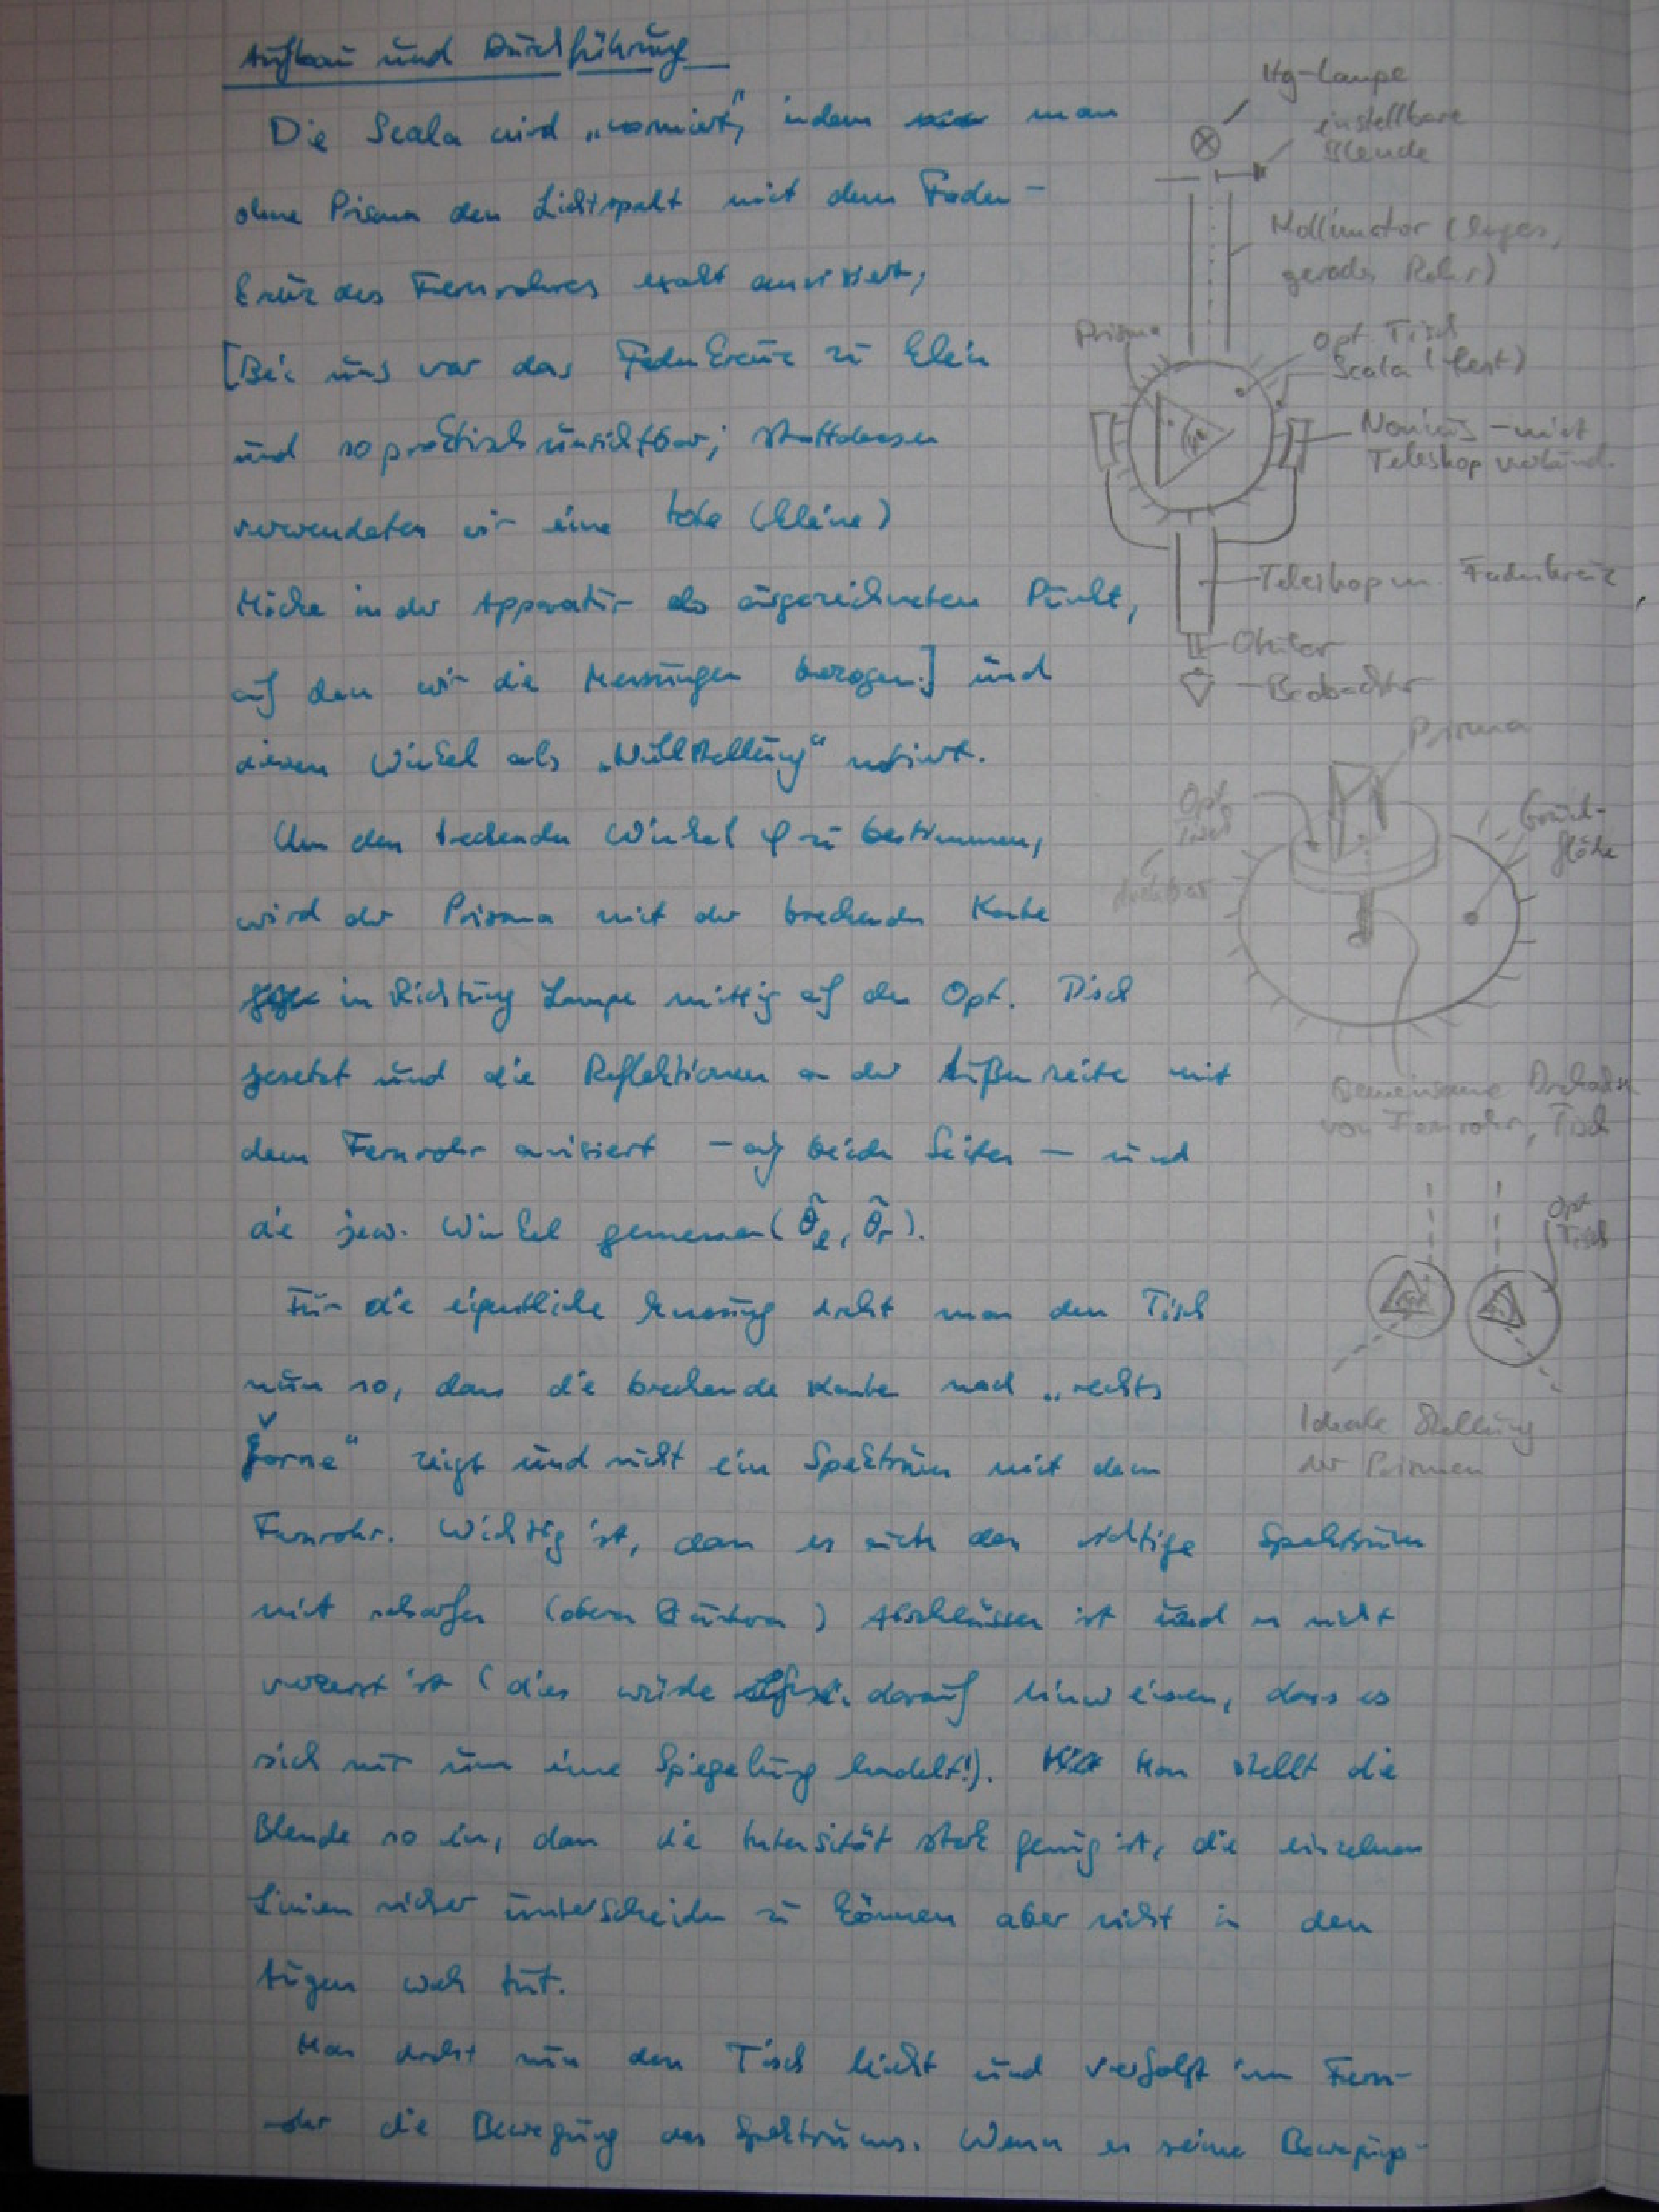
\includegraphics[width=0.8\textwidth]{aufbau}
  \caption{Aufbau des ESR-Versuchs. Blau durchgezogen ist die
    einlaufende Mikrowelle, die Reflektierte ist gr"un. Gestrichelt
    sind die Mikrowellen gezeichnet, die absorbiert werden.}
  \label{fig:aufbau_esr}
\end{figure}


In Abb. \ref{fig:aufbau_esr} ist der Aufbau des ESR-Versuchs
Schematisch aufgezeichnet. Auch hier werden die Mikrowellen mittels
eines Klystrons erzeugt und in Hohlleitern transportiert. Der
Einwegeleiter direkt dahinter verhindert, dass reflektierte
Mikrowellen wieder in das Klystron gelangen.

Ein kleiner Teil der erzeugten Mikrowellen wird ausgekoppelt (dazu
liegen zwei Hohlleiter direkt nebeneinander und sind an bestimmten
Stellen durchbrochen und dadurch verbunden) und die Frequenz wird
gemessen (vgl. Kap. \ref{sec:messung_der_mikrowellenfrequenz}).

Der Rest l"auft durch einen einstellbaren D"ampfer (damit die Diode
keine zu starken Intensit"aten abbekommt) zu einem
sog. \emph{Magischen T}. Durch seine spezielle Bauart werden die
Mikrowellen zu gleichen Teilen in zwei verschiedene, entgegengesetzte,
Richtungen geleitet: Der eine Teil wird in einem Wellensumpf
vernichtet (die Mikrowelle wird praktisch ohne Reflektion absorbiert),
der andere Teil l"auft in den Messresonator.

Dieser steht zwischen zwei Lorentzspulen, die ein homogenes Magnetfeld
$\vec B_0$ darin erzeugen. Zudem sind zwei kleien Spulen angebracht,
die das gro"se B-Feld $\vec B_0$ leicht variiertn -- dies ist wichtig
f"ur die Messung; vgl Kap. \ref{sec:lock_in_messverfahren}. Die
St"arke des Magnetfelds im Resonator wird durch eine Hallsonde gemessen.

Die Mikrowellen, die den Resonator wieder verlassen, kommen wieder in
das Magische T, wo sie so aufgeteilt werden, dass die H"alfte im
Wellensumpf absorbiert wird und die andere H"alfte gelangt in eine
Messdiode. Die hier gemessenen Daten werden demoduliert (vgl wieder
Kap. \ref{sec:lock_in_messverfahren}) und am Komputer auf die
$y$-Achse der Diagramme aufgetragen, die $x$-Achse bildet die
Spannung, die an der Hallsonde anliegt und proportional zum B-Feld
im Resonator ist.


\subsection{Lock-In-Messverfahren}
\label{sec:lock_in_messverfahren}


Mit den beiden in Kap. \ref{sec:aufbau} erw"ahnten kleinen Spulen wird
das Magnetfeld $\vec B_0$ leicht -- sinusf"ormig -- variiert.
Frequenz und Amplitude der Variation geh"oren zu den sp"ater zu
optimierenden Parametern.

In Abb. \ref{fig:modulation_b-feld} ist skizziert, wie sich die
Modulation des B-Feldes auswirkt: Die gro"se Kurve ist die
Absorptionskurve \footnote{Eigentlich m"usste die Kurve nach unten
  zeigen, weil ja bei Absorption das Diodensignal kleiner wird. Die
  Vorzeichenumkehr ist ein technischer Effekt des Lock-In-Amplifiers.}
der Probe aufgetragen "uber das B-Feld. Unten sieht man die Variation
des Signals an einer Stelle (gestrichelte Linie) mit bestimmter
Amplitude (durchgezogene Linie). Hier ist die Vertikale eine
Zeitachse. An der Kurve sieht man jeweils nach rechts das Signal
weglaufen, das generiert wird -- hier ist die Horizontale eine
Zeitachse. Hier ist die Amplitude des Signals dadurch bestimmt, wie
steil die Absorptionskurve an der Stelle der vertikalen gestrichelten
Linie ist -- deshalb erh"alt man in den Plots stets die
\emph{differenzielle} Absorptionskurve, weil man stets die Steigung,
also die Ableitung, der eigentlichen Kurve misst.

\begin{figure}[!h]
  \centering
  \includegraphics[width=0.6\textwidth]{modulation}
  \caption{Messverfahren: Modulation des B-Feldes. Bild von Bietsch,
    W. und W. Hartl: Elektronenspinresonanz (ESR)}
  \label{fig:modulation_b-feld}
\end{figure}


Wichtig ist jetzt noch, dass die Signale, die nach rechts weglaufen
zeitlich gemittelt werden. Im Endeffekt erh"alt man dadurch die
horizontalen gestrichelten Linien. Dies ist die Demodulation des
aufmodulierten Signals.  Dadurch sinkt die Aufl"osegenauigkeit -- und
es steigt die Linienbreite -- wenn man eine gro"se Amplitude
verwendet, weil die Mittlung "uber einen gr"o"seren B-Feld-Bereich
geht.




\subsection{Automatic Frequenzy Control (AFC)}
\label{sec:automatic_frequenzy_control}


Bei dem Versuch ist es wichtig, dass die Mikrowellenfrequenz
m"oglichst konstant ist. Wir verwenden deshalb ein sog. AFC. 
% Man muss
% es zu Beginn des Versuchs einstellen: Wie auch der Frequenzmesser
% erzeugt auch das AFC einen (deutlich gr"o"seren) Dip in einem
% $U_\text{Reflektor}$-$P_\text{Diode}$-Diagramm. 
Das Klystron muss so feinabgestimmt werden, dass es in einem
$U_\text{Reflektor}$-$P_\text{Diode}$-Diagramm ein symmetrisches
Minimum hat. Das Minimum kommt durch Absorption im Resonator
zustande. "`Symmetrisch"' bedeutet hier, dass die Maxima neben dem
Minimum gleich hoch sein sollen und dass die "`H"ange"' des Minimums
auf beiden Seiten m"oglichst gleich sind.
Das AFC "`erkennt"' dann das Minimum und sobald das
Klystron von der Frequenz abweicht, wird seine Reflektorspannung
leicht angepasst um es wieder auf die richtige Frequenz zu bringen.

Das Klystron muss derartig jedesmal abgestimmt werden, wenn eine Probe
gewechselt wurde (oder aus sonstigen Gr"unden die D"ampfung zu hoch
war als dass die hintere Diode das AFC hinreichend mit Daten versorgen
konnte). Auch ist es wichtig, vor jeder Messung zu "uberpr"ufen, ob
das Klystron seine Frequenz h"alt, weil die Messung sonst keine
sinnvollen Daten liefert.










\section{Mikrowelle}
\label{sec:mikrowelle}





\subsection{Kennlinie der Detektordiode}
\label{sec:kennlinie_der_detektordiode}

\begin{figure}[!h]
  \centering
 \includegraphics[angle=-90,width=0.9\textwidth]{../data/mikrowellen/daempf-diode-1} 
  \caption{Kennlinie der Detektordiode -- tats"achliche "uber gemessene D"ampfung}
  \label{fig:kennlinie_detektordiode}
\end{figure}


In Abb. \ref{fig:kennlinie_detektordiode} sieht man, dass die
gemessene mit der tats"achlinen D"ampfung linear zusammenh"angt --
allerdings mit zwei verschiedenen Linearit"aten (deshalb auch zwei
verschiedene lineare Fits).

Erwartet h"atten wir einen einfacheren linearen Zusammenhang.  Dass es
sich nicht um eine Ursprungsgerade handelt, ist 
% --
durch die logarithmische Auftragung der D"ampfung 
% --
nicht weiter
verwunderlich.
%, weil die Diode
% als Referenzwert einen Wert direkt
% hinter dem Klystron verwendet und so die Verluste in der Leitung
% zwischen Klystron und Diode nicht einkalkuliert.



Interessant ist auch, dass keine der beiden Geraden parallel zu
$f(x)=x$ ist. Selbst wenn man den Offset ($y$-Achsenabschnitt) der
Messwerte verschiebt, so erh"alt man in keinem Messbereich die
korrekte D"ampfung direkt von der Diode angezeigt.

%  also dass auch durch Nachregulieren einer der beiden
% Fits auf eine Ursprungsgerade die beiden Methoden nicht das selbe
% Ergebnis bringen. 

% Das kann aber (auch)  daran liegen, dass bei der
% Messung mit den Signalh"ornern mehr
% Mikrowellen an dem Zweiten Signalhorn vorbei in den Raum abgegeben
% werden je senkrechter die beiden H"orner aufeinander stehen.

Im ersten -- kleinen -- Kennlinienbereich gibt die Messung mit Diode eine zu
niedrige D"ampfung an; sie misst also eine zu hohe
Intensit"at. 
% M"oglicherweise hat dies einfach mit der Bauart der Diode
% zu tun, dass man hier f"ur hohe Intensit"aten schon im
% Solarzellenbereich ist.

Beachtet man, dass wir bei den Messungen stets mit logarithmischen
Gr"o"sen rechnen, so kann man sich den Kurvenverlauf auch quantitativ
erkl"aren: Der erste "`steilere"' Bereich ist der "`quadratische"'
Bereich der Diode, dahinter geht sie in den Proportionalbereich
"uber. Durch die Logarithmierung entsprechen diese Potenzen den
Steigungen der Kurve.





\subsection{Kalibrierkurve Foliend"ampfer}
\label{sec:kalibrierkurve_foliendampfer}

\begin{figure}[!h]
  \centering
 \includegraphics[angle=-90,width=0.9\textwidth]{../data/mikrowellen/daempf-folie-1} 
  \caption{Kalibrierkurve des Foliend"ampfers -- Tats"achliche
    D"ampfung "uber Eintauchtiefe}
  \label{fig:kalibrierkurve_folie}
\end{figure}


In Abb. \ref{fig:kalibrierkurve_folie} ist die Kalibrierkurve des
Foliend"ampfers aufgenommen. Im Bereich f"ur nur wenig eingeschobene
Folie ist die D"ampfung quadratisch angefittet, f"ur st"arker
eingeschobene Folie linear. Ab ca. 5mm Eintauchtiefe der Folie ist
dieser lineare Fit nicht mehr g"ultig.

\begin{figure}[!h]
  \centering
 \includegraphics[angle=-90,width=0.9\textwidth]{../data/mikrowellen/daempf-folie2-1} 
  \caption{Kalibrierkurve des Foliend"ampfers -- Tats"achliche
    D"ampfung "uber Eintauchtiefe.}
  \label{fig:kalibrierkurve_folie_logistisch}
\end{figure}



In Abb. \ref{fig:kalibrierkurve_folie_logistisch} ist zum Vergleich
eine logistische Kurve angefittet. Offensichtlich passt sie wesentlich
besser zu dem Messwerten; die Fits in
Abb. \ref{fig:kalibrierkurve_folie} sind gewisserma"sen die
Taylorentwicklung der besseren Kurve. Die logistische Kurve hat die Vorschrift
\begin{equation}
\label{eq:kalibr_foliendaempfer}
  D(x) =
\frac{ 63.49852 }{ 1 + \exp( - 1.026462 * ( x - 3.897382 ) ) } \;.
\end{equation}

Die Eintauchtiefe bezeichnet hier den Abstand der parallelen
leitf"ahigen Folie von der Au"senwand. Innerhalb des Hohlleiters ist
die E-Feld-Verteilung theoretisch im Idealfall eine Sinuskurve (also
$E = E_0 \, sin(x)$, wobei $x$ die Entfernung von der Wand ist). In
der Praxis wird es zu einem "ahnlichen Verlauf kommen.

Ist der Foliend"ampfer komplett eingefahren, so liegt an ihm nur ein
sehr kleines E-Feld vor, was von Randbedingungen im Hohlleiter
diktiert wird. Damit sind die ohmschen Verluste in der Folie
auch nur sehr klein ($P_\text{Verlust} \propto E^2$). Je weiter das
F"ahnchen in die Mitte geht, desto gr"o"ser ist hier das E-Feld und
damit die ohmschen Verluste und damit auch die D"ampfung. Das E-Feld
steigt stark an -- ebenso also die D"ampfung und damit unsere Kurve --
und geht schlie"slich in einen S"attigungsbereich "uber. Hier hat
eine Verschiebung der D"ampfungsfolie dann immer weniger Effekt.

\begin{figure}[!h]
  \centering
 \includegraphics[angle=-90,width=0.9\textwidth]{../data/mikrowellen/daempf-folie3-4} 
  \caption{Kalibrierkurve des Foliend"ampfers -- Tats"achliche
    D"ampfung "uber Eintauchtiefe. Hier ist einmal eine logistische
    Kurve angefittet -- weil die Messwerte eben so aussehen -- und
    eine Theoriekurve, die die Wellenverteilung im Leiter zugrundelegt.}
  \label{fig:kalibrierkurve_folie_sinus}
\end{figure}

Eine durch diese "Uberlegung erhaltene Kurve ist ebenfalls in
Abb. \ref{fig:kalibrierkurve_folie_sinus} angegeben. Man sieht (an den
Boxen -- sie geben die Abweichung von den Messwerten an),
dass sie f"ur die "`mittleren"' Werte -- also Eintauchtiefen zwischen
$2\operatorname{mm}$ und $8\operatorname{mm}$ -- eine sehr gute "Ubereinstimmung
mit den Messweten zeigt, am Rande jedoch nicht mehr
"ubereinstimmt. Dies liegt vermutlich daran, dass in der Realit"at das
E-Feld nicht wirklich auf $0 \operatorname{V}/\operatorname{m}$
abf"allt -- au"serdem hat auch hier der Foliend"ampfer eine d"ampfende
Wirkun, weil er eine endliche Dicke hat. 

M"ochte man die Kallibrierkurve als "`Arbeitswerkzeug"' verwenden --
also nur um die tats"achliche D"ampfung herauszubekommen, wenn man die
Eintauchtiefe kennt -- so kann man getrost
\eqref{eq:kalibr_foliendaempfer} verwenden. Die Theoriekurve
verifiziert die zugrundegelegte Theorie.





\subsection{Charakteristik der Klystronmoden}
\label{sec:charakteristik_der_klystronmoden}


\begin{figure}[!h]
  \centering
 \includegraphics[angle=-90,width=0.9\textwidth]{../data/mikrowellen/mode123-2} 
  \caption{"Ubersicht "uber die Klystronmoden mit Leistung und
    Frequenzen "uber Spannung}
  \label{fig:klystronmoden_uebersicht}
\end{figure}




Abb. \ref{fig:klystronmoden_uebersicht} zeigt eine "Ubersicht
"uber die einzelnen Moden, in Abb. \ref{fig:klystronmoden_einzeln} sind sie
nochmal einzeln aufgef"uhrt.

\begin{figure}[!h]
  \centering
  \subfigure[]{\includegraphics[angle=-90,width=0.40\textwidth]{../data/mikrowellen/mode1-2}}
  \subfigure[]{\includegraphics[angle=-90,width=0.40\textwidth]{../data/mikrowellen/mode2-2}}
  \subfigure[]{\includegraphics[angle=-90,width=0.40\textwidth]{../data/mikrowellen/mode3-2}}
  \caption{Die drei Moden einzeln}
  \label{fig:klystronmoden_einzeln}
\end{figure}






Wir bestimmen die Bandbreite stets als FWHM (vgl
Kap. \ref{sec:fitten}) der Amplitude.

Die Abstimmempfindlichkeit $A$ geben wir als
\begin{equation}
  \label{eq:def_abstimmempfindlichkeit}
  A = \frac{ \Delta \nu } { \Delta U }
\end{equation}
an.
 
So ergeben sich die folgenden Gr"o"sen (abgelesen aus den Schaubildern):

\begin{tabular}{ r  r  r  r }
  Spannung bei Maximum [V] & $\Delta \nu$ [MHz] &   $\Delta U$ [V] &  $A$ [MHz/V] \\
     175.0 & 99.1 &  31.4 & 3.14 \\
     121.4  & 124.1 & 22.4 & 5.54 \\
     80.4  &  122.0  & 15.0 & 8.13
\end{tabular}

Man sieht deutlich, die Abstimmgenauigkeit bei gro"sen Spannungen
besser ist, ebenso ist hier
(Vgl. Abb. \ref{fig:klystronmoden_uebersicht}) die absolut erreichbare
Leistung am gr"o"sten.







\subsection{Wellenl"angen im Leiter}
\label{sec:wellenlangen_im_leiter}




Es ist experimentell sinnvoller, ein Maximum zu suchen, das SWR auf
diese D"ampfung eingestellt zu lassen, und dann mit dem Stehwellen-Detektor
weitere Maxima zu suchen. Anschlie"send stellt man den Stehwellen-Detektor
und damit auch das SWR auf ein Minimum ein und bestimmt alle Mimima
nacheinander.

Wir haben jetzt zu beachten, dass die Intensit"at mit $I \propto E^2$
geht. D.h. wenn wir den Abstand zwischen zwei Maxima bzw. zwischen
zwei Minima berechnen, so bekommen wir nicht die Wellenl"ange, sondern
nur die \emph{halbe} Wellenl"ange, weil $E \propto \cos(y) \folgt I
\propto \cos^2(y)$.

Nach Auswertung aller -- verwertbaren --
Daten\footnote{Offensichtliche Ausrei"ser wurden gestrichen} erh"alt
man
\begin{equation}
  \label{eq:1}
%  \lambda_h \approx 25.14 \operatorname{mm} \pm 1.38 
% \operatorname{mm}  \;,
  \lambda_h = 50.28 \operatorname{mm} \pm 2.76 \operatorname{mm} \;,
\end{equation}
wobei "`$\pm$"' stets die mittlere Abweichung vom Mittelwert angibt.


Zur Kontrolle haben wir die Messung noch mit Oszilloskop und einer
sinusf"ormigen Reflektorspannung durchgef"uhrt. Dies hat den Vorteil,
dass wir an einem Oszilloskop direkt die Spannung des Reflektors
($x$-Achse) und der Diode ($y$-Achse) anschlie"sen konnten. Hier kann
man beim verschieben des Frequenzmessers einen kleinen Dip wandern
sehen und diesen so gut auf die Frequenz einstellen, au"serdem die
Maxima und Minima besser beobachten als im SWR-Meter, weil dieses bei
unserem Versuch sehr stark geschwankt hat, sodass man nicht sicher
sein konnte, ob man sich wirklich an einem Minimum befindet oder ob
gerade nur der Messzeiger schwankt. Die so erhaltene Wellenl"ange
\begin{equation}
  \label{eq:2}
%  \lambda_h^{\sin} \approx 24.17\operatorname{mm} \pm
%  0.96\operatorname{mm} \;.
  \lambda_h^{\sin} = 48.34\operatorname{mm} \pm
  1.92\operatorname{mm} \;.
\end{equation}
ist einfach ein Vergleichswert f"ur die Gr"o"senordnung.


Die Frequenz, bei der wir diese Versuche durchgef"uhrt haben, lag bei
ca.
\begin{equation*}
  \nu = 9109.5 \operatorname{MHz}
\end{equation*}
was einer Vakuumwellenl"ange (wir nehmen an, dass $c_\text{Luft} = 1$
gilt) von
\begin{equation*}
  \lambda_0 = \frac c \nu = 32.9 \operatorname{mm}
\end{equation*}
entspricht.



Bei uns handelt es sich vermutlich um eine Grundmode, also $m=1$ und
$n=0$. Aus den Din-Norm-Bestimmungen des Wellenleiters ("`R100"')
folgt
\begin{equation*}
  a = 22.869 \operatorname{mm} \text{ und } b =
  10.160\operatorname{mm} \;.
\end{equation*}
Berechnet man mit diesen Werten aus \eqref{eq:5} $\lambda_H$ f"ur
$m=1$ und $n=0$, so erh"alt man
\begin{equation*}
  \lambda_H = 47.38\operatorname{mm} \;.
\end{equation*}

Dass es sich um eine andere Mode als die angenommene handelt kann man
ausschlie"sen, weil f"ur gr"o"sere $m,n$ die Wurzel stets negativ wird
und damit $\lambda_H \notin \mathbb R$.

Wir haben damit eine Differenz zwischen den aus der Frequenz
berechneten und den gemessenen Werten von
\begin{equation*}
  \text{absolut: } \Delta \lambda_h = 0.96\operatorname{mm} \text{ und
    relativ: } \delta \lambda_h = \frac{ \Delta \lambda_h }{ \bar
    \lambda_h } = 0.020 \;,
\end{equation*}
wobei wir die Messwerte aus der Sinus-Messung verwendet haben, 
% weil
% die Herleitung von \eqref{eq:5} diese Gestalt zugrundelegt.
weil wir hier genauer (als mit dem stark schwankenden SWR-Meter)
bestimmen konnten, wann wir ein Maximum und wann wir ein Minimum an
der Sonde haben.

Die Abweichung zwischen dem Theoretischen und dem Gemessenen Wert
liegt offenbar innerhalb der Genauigkeit von $\lambda_h$, weswegen wir
damit eigentlich gl"ucklich sein k"onnen.







 

 
 \subsection{Stehwellenverh"altnis}
 \label{sec:stehwellenverhaltnis}

Wir konnten nur die Versuche mit Kurzschluss durchf"uhren. Beim
Wellensump konnten wir keine stehenden Wellen nachweisen: Die
Ausschl"age gingen im Rauschen unter. Mit dem Wellensumpf konnten wir
lediglich die Frequenz $\nu \approx 9042.0 \operatorname{MHz}$
bestimmen.




 \subsubsection{3dB-Methode}
 \label{sec:3db_methode}



Ein Minimum lag bei $68.72\operatorname{mm}$ und
$24.55\operatorname{dB}$. Der Wert $24.55\operatorname{dB} - 10 \, \lg
2 \approx 21.54\operatorname{dB}$ wurde angenommen bei 
\begin{equation*}
  d_1 = 79.4 \operatorname{mm} \text{ und } d_2 =
  79.64\operatorname{mm} \folgt \Delta d = 0.24\operatorname{mm}\;.
\end{equation*}
Damit folgt mit
% \footnote{Hier haben wir die Wellenl"ange der Welle
%   verwendet, die mit  der rechteckigen Reflektorspannung  erzeugt
%   wurde.} 
$\lambda_h = 50.28\operatorname{mm}$ aus
Kap. \ref{sec:wellenlangen_im_leiter}, eingesetzt in Gl. \eqref{eq:27}
\begin{equation*}
  S = \sqrt{ 1 + \frac 1 {\sin^2 \frac{ \pi \, \Delta d } { \lambda_h
      } } } = 66.70 \;.
\end{equation*}




Leider ist in dieser Messung ein Fehler, weil wir beim Versuch
selbst die Kalibrierkurve f"ur die Diode h"atten verwenden
m"ussen. Doch der Fehler ist nicht besonders gro"s, weil f"ur diese
Werte ("uber 14dB) der zweite lineare Fit aus Abb.
\ref{fig:kennlinie_detektordiode} g"ultig ist und dieser nur wenig von
der Identit"at $f(x) = x$ abweicht.


\subsubsection{SWR-Meter-Methode}
\label{sec:swr_meter_methode}


Das Maximum lag bei $10.70\operatorname{dB}$, das Minimum bei
$24.55\operatorname{dB}$; es folgt aus Gl. \eqref{eq:3}
\begin{equation}
  S = 10^{ \frac{ D_\text{max} - D_\text{min} } {20} } = 4.93 \;.
\end{equation}


Hier haben wir aber noch auf die Angaben der Diode vertraut. Liest man
aus Abb. \ref{fig:kennlinie_detektordiode} die korrekten Werte ab, so
bekommt man mit $D'_\text{max} = 7.97\operatorname{dB}$ und
$D'_\text{min} = 29.07$ den neuen Wert
\begin{equation*}
  S' = 10^{ \frac{ D'_\text{max} - D'_\text{min} } {20} } =
  11.35 \;.
\end{equation*}



\subsubsection{Abschw"achungsmethode}
\label{sec:abschwachungsmethode}


% Aus Kalibrierkurve f"ur Foliend"ampfer folgt f"ur $x_0 =
% 0\operatorname{mm}$ und $x_1 = 4.46\operatorname{mm}$ mit \eqref{eq:3}
% \begin{equation*}
%   S \sim 1.0 \;.
% \end{equation*}

Sucht man bei abgeschalteter D"ampfung ($x_0=0\operatorname{mm}$) ein
Maximum und ein Minumum und d"ampft dann mit dem Foliend"ampfer das
Maximum (also mit der Messsonde auf das Maximum eingestellt) so
lange, bis man den Wert des Minumums erhalten hat -- der
Foliend"ampfer hat dann die Eintauchtiefe $x_1 =
4.46\operatorname{mm}$ -- so kann man mit Gl. \eqref{eq:3} wieder $S$
berechnen, indem man mit der aus dem Fit gewonnenen Gleichung
\eqref{eq:kalibr_foliendaempfer} die jew. D"ampfungen bestimmt. Diese
sind $D_\text{max} = 0\operatorname{dB}$ und $D_\text{min} = 40.67\operatorname{dB}$ Es
gilt dann
\begin{equation*}
  S = 108.01 \;.
\end{equation*}


 

\subsubsection{Vergleich der Methoden}
\label{sec:vergleich_der_methoden}

Die direkte Messmethode (also SWR-Meter-Methode) eignet sich gut f"ur
Messungen im "`quadratischen"' Bereich der Diode. Dies ist bei uns der
steile Bereich bis zu gemessenen 14dB.
 Damit ist diese Methode gut
f"ur kleine SWR geeignet. 

% Problematisch kann hier sein, dass die Sonde
% im Maximum "uberlastet ist und dadurch weniger genau misst.

Bei zu gro"sen SWR kann die Leistung an der Detektordiode so hoch
sein, dass diese nicht mehr im quadratischen Bereich arbeitet. 

Um diese "`"Uberlastung"' zu "uberwinden verwendet man die
3-dB-Medhode. 
Bei dieser muss die Diode nicht mehr
im quadratischen Bereich arbeiten liegen (also "uber 14dB). Damit
eignet sie sich am besten f"ur die Messung gro"ser SWR. 
% Da man hier
% aber au"serhalb des quadratischen Bereichs arbeitet, kommen gewissen
% Abweichungen hinzu. Um diese auszuschalten verwendet man die Abschw"acher-Methode 

Die Abschw"achungsmethode versucht, Fehler auszum"arzen, die sich
dadurch ergeben, dass man nicht mehr im quadratischen Bereich der
Sonde arbeitet. Der Fehler dieser Methode h"angt von der Genauigkeit
des (Folien)D"ampfers ab. Hiermit kann man gro"se SWR bestimmen.


 



\subsubsection{Mit Anpassung durch Gleitschraubentransformator}
\label{sec:mit_anpass_durch_gleitschr}

Nach einiger Suche konnten wir eine Eintauchtiefe $z =
10.0\operatorname{mm}$ und $y = 96.9\operatorname{mm}$ finden, sodass
sich bei Fehlanpassung des Exponentialhornes auf der ganzen Reichweite
des Stehwellendetektors die Messwerte nur wenig "anderten: Ein Maximum
lag im Oszilloskop bei $0.50\operatorname{V}$, ein Minimum bei
$0.21\operatorname{V}$, also einer Differenz von $\Delta U =
0.29\operatorname{V}$.

 
 
 
 





\section{ESR-Spektroskopien}





\subsection{Resonatorg"ute}
\label{sec:resonatorgute}



Die G"ute des Resonators \inh{ohne eingebaute Proben} ist (Berechnung
stets nach \eqref{eq:guete_def}):
\begin{equation*}
	Q^\text{leer} = 2164.7  \text{ bei }
        \nu_0 = 9.525\operatorname{GHz}\;.
\end{equation*}

Die G"ute des Resonators mit der eingesetzten Probe \inh{"`polykristallines DPPH"'} ist
\begin{equation*}
	Q^\text{DPPH} = 2058.9 \text{ bei } \nu_0 = 9.514 \operatorname{GHz}\;,
\end{equation*}
also wird die G"ute durch das Einf"uhren der Probe nur leicht
verschlechtert.

F"ur \inh{polykristallines Kupfersulfat} ist die G"ute
\begin{equation*}
%  Q^{\operatorname{Cu}^{2+}} = 2314.6 \;,
  Q^{\operatorname{Cu}^{2+}} = 2245.6 \text{ bei } \nu_0 = 9.514 \operatorname{GHz}\;,
\end{equation*}
also etwas besser als ohne Probe 
und f"ur \inh{w"assrige Mangan-II-L"osung}  
\begin{equation*}
  Q^{\operatorname{Mn}^{2+}} = 2060.4 \text{ bei } \nu_0 = 9.523 \operatorname{GHz}\;,
\end{equation*}
also wieder so wie beim DPPH.


\abs
Wenn die Probe im Resonator Mikrowellenenergie absorbiert, so
verringert sich $Q$, weil die "`Energieverluste"' gr"o"ser sind --
vgl. Gl. \eqref{eq:4}. Wir sind deshalb etwas verwirrt, dass die G"ute
mit der Kupferprobe  besser ausgefallen ist. 

Ebenfalls interessant ist, dass eine Probe eigentlich die
Impedanz des Resonators "andert und dadurch ergibt sich eine neue
Resonanzfrequenz. Diese muss man einstellen, um weiterhin kritisch zu
koppeln. Bei der Mangan-L"osung haben wir jedoch praktisch die selbe
Frequenz wie beim leeren Resonator und trotzdem ist die G"ute anders.

\abs
%
Um zu sehen wie relevant unsere Ergebnisse sind ist nun eine
Fehlerrechnung unabdingbar.  In diese wird die Umrechnungsfunktion
einbezogen, welche uns den Wert welchen wir vom Frequenzmesser ablesen
in unsere wahre Frequenz umrechnet:
\begin{equation}
  \nu = {K - c \cdot x} \;,
\end{equation}
wobei hier $x_0$ der an der Mikrometerschraube abgelesene Wert (in mm)
von $\nu_0$, usw. ist, $K = 10.529\operatorname{GHz}$ und $c =
0,1284\operatorname{GHz}/\operatorname{mm}$.

Diese Formel wird dann in Gleichung \eqref{eq:guete_def} eingesetzt
und man erh"alt:
\begin{equation}
	Q = \frac{K - c x_0}{| c ( x_r - x_l ) |}
\end{equation}

Da man davon ausgehen kann, dass beim Bestimmten von $x$ jeweils (beim
Oszilloskop und Frequenzmesser) ein Fehler mindestens in der letzten
Nachkommastelle gemacht wurde geht man von $\Delta x =
0.003\operatorname{GHz}$ aus. Bei den Werten aus der Umrechnungsformel
kann man ebenfalls von einem Fehler in der letzten bestimmten Stelle
ausgehen, daher $\Delta K = 0.001\operatorname{GHz}$ und $\Delta c
= 0.0001\operatorname{GHz}/\operatorname{mm}$.

Die sich ergebende Feherfortpflanzung f"ur $Q$ lautet dann
\begin{equation}
	\Delta Q = \frac{K}{c^2 (x_r - x_l)} {\Delta c} + \left(
        \frac{1}{x_r - x_l} + \frac{2 (K - c x_0)}{c (x_r - x_l)^2}\right)
        {\Delta x} + \frac{\Delta K}{c (x_r - x_l)} \;.
\end{equation}

Daraus ergeben sich dann folgende Werte:
\begin{eqnarray*}
\Delta Q^\text{leer} &=& 416.5 \\
\Delta Q^\text{DPPH} &=& 327.9 \\
\Delta Q^\text{Cu} &=& 467.7 \\ 
\Delta Q^\text{Mn} &=& 373.1 \;.
\end{eqnarray*}

Damit k"onnen die ungew"ohnlichen Ergebnisse von oben leicht durch
Fehler erkl"art werden. Die Aussage der Messung der Resonatorg"ute
bel"auft sich so allerdings dann darauf, dass sie sich beim Einsetzten
verschiedener Proben nicht weitl"aufig "andert.




\abs
F"ur die G"ute gilt
\begin{equation}
  \label{eq:6}
  Q = \frac{ 1 } { \frac{1}{Q_0} + \frac{1}{Q_s} } \text{ mit } Q_s =
  \frac{1}{4\pi \eta \chi'' }
\end{equation}
D.h. sie addiert sich wie parallele Wiederst"ande aus den G"uten von
leerem Resonator $Q_0$ und der Probe $Q_s$. In der zweiten Formel ist
nun  $\eta$ der Filling-Factor (gibt an, welchen Anteil des Resonators
die Probe belegt)
und $\chi''$ die Mikrowellen-Suszeptibilit"at des Materials.

F"ur uns entscheidend ist, dass diese Gr"o"sen von der
\emph{Relaxationszeit} $T_2$ der Ausrichtung von $\vec \mu$ im B-Feld
abh"angen.







\subsection{Bestimmung guter Parameter des ESR-Aufbaus}
\label{sec:bestimmung_guter_parameter}


Um eine optimale Konfiguration zu erhalten, hatten wir folgende Idee: 
\begin{enumerate}
\item 
Wir setzen alle Parameter so, dass der "`interessante"' Bereich der Kurve auf dem
Bildschirm liegt (also insbesondere muss die D"ampfung so eingestellt werden,
dass die y-Achse nicht "uberschritten wird, also alle Messwerte innerhalb
$\pm10$ liegen).

Hier kann man schon sehen, dass man -- wie erwartet -- die Kurvenh"ohe
durch die D"amfung einstellen kann:
Vgl. Abb. \ref{fig:kleiner_bei_daempfung}.\footnote{F"ur die
  Verschiebung der Kurve nach links siehe Absatz unten.}
\item 
%
  Nur die Frequenz der Magnetfeldmodulation wird ver"andert und die
  optimale Frequenz wird bestimmt. Wir haben dabei versucht die
  D"ampfung so anzupassen, dass wir weiterhin den Messbereich
  weitgehend ausnutzen.

Bei uns sah es so aus als w"urden kleine Frequenzen
sch"arfere Kurven ergeben. Siehe Abb. \ref{fig:duenner_bei_frequenz}.
Als gute Frequenz haben wir so $\nu = 20
kHz$ bestimmt.

Was wir nicht beachtet haben, war die Tatsache, dass bei anderen
Stoffen der Amplitudenausschlag bei Resonanz auch bei abgeschalteter
D"ampfung sehr gering sein kann, d.h. dass auch noch so sch"on schmale
(d.h. scharfe) Kurven uns wenig bringen, wenn sie in der Intensit"at
so schwach sind, dass sie im Rauschen untergehen. In
\ref{fig:kleiner_bei_frequenz} sieht man, dass die Amplitude bei
gro"sen Frequenzen abnimmt. (Vgl. Kap. \ref{sec:einfluss_der_parameter}.)
% R"uckblickend muss man sagen, dass wir
% mehr Wert auf eine gute Amplitude h"atten legen m"ussen.
\item 
Anschlie"send haben wir die Amplitude des aufmodulierten
B-Feldes\footnote{Bzw. eigentlich die Amplitude der
  Ansteuerungsspannung des B-Feldes} variiert und dabei die D"ampfung
wieder so angepasst, um den Messbereich wieder weitestgehend
auszunutzen. Bei kleinen Amplituden hatten wir scharfe Linien -- vlg. \ref{fig:duenner_bei_ampl}.

Den sch"arfsten Peak haben wir bei ca. $A = 3\operatorname{V}$
ermittelt.
\item Dann haben wir die Integrationszeit variiert.\footnote{Im
    Programm muss man entsprechend den Delay anpassen: Ist der Delay
    kleiner als die Integrationszeit, so macht das keinen Sinn, weil
    dann mehrmals Daten abgefragt werden, obwohl das Messger"at noch
    beim selben auszugebenden Wert beim integrieren ist -- also der
    selbe Wert mehrfach aufgenommen wird.} Hier sieht man lediglich,
  dass bei kleiner Integrationsdauer die Kurve st"arker verwackelt
  ist. Vlg. Abb. \ref{fig:integrationszeit} Bei sehr gro"ser Dauer
  w"urde die Kurve wohl verschmieren, so gro"se Zeiten konnten wir
  aber gar nicht einstellen. Um auf Nummer sicher zu gehen haben wir
  eine recht kurze Integrationszeit gew"ahlt.
\end{enumerate}

Insgesamt ergaben sich hier als beste Einstellungen:
\begin{eqnarray*}
  \text{Frequenz der Modulation: } & 20\operatorname{kHz}\\
  \text{Amplitude der Modulation: } & 3\operatorname{V}\\
  \text{Integrationszeit: } & 30\operatorname{ms}\\
  \text{D"ampfung: } & 7\operatorname{dB}
\end{eqnarray*}



Leider ergab sich, nachdem wir lange die verschiedenen Einstellungen
durchvariiert hatten, dass die Kurven sich auch v"ollig ohne unser
zutun ver"anderten -- vgl Abb. \ref{fig:wandern_bei_temp}. Woran genau
das liegt k"onnen wir nicht sagen, es war an dem entsprechenden
Versuchstag aber sehr hei"s bei uns. M"ochlicherweise hat sich also
bspw. ein bestimmtes Bauteil aufgeheizt und verbogen etc. 

% Fakt ist jedenfalls, dass wir unsere Einstellungen bei den weiteren Messungen
% variieren mussten, um verwertbare Daten zu erhalten, sodass diese
% Anpassung leider nicht besonders sinnvoll war...

Die Parameter die wir gefunden haben, sollten eine m"oglichst kleine
Linienbreite der Kurven erm"oglichen. F"ur manche Messungen war
dadurch aber die Amplitude des Messsignals so viel zu klein, dass die
Messungen im Rauschen untergingen. Dann mussten wir Parameter so
ab"andern, dass wir noch einen Linienverlauf durch das Rauschen sehen
konnten -- entsprechend vergr"o"serte sich hier aber die Linienbreite.


\begin{figure}[!h]
  \centering
  \subfigure[Amplitudenmudulationsfrequenz $f$ bei ausgeglichener
  D"ampfung (angegeben $T = 1/f$)]{\includegraphics[angle=-90,width=0.40\textwidth]{../data/spektren/polyDPPH/vary_freq/duenner_bei_frquenz}\label{fig:duenner_bei_frequenz}}
  \subfigure[Amplitudenmudulationsfrequenz $f$ ohne ausgleichende
  D"ampfung (angegeben $T =
  1/f$)]{\includegraphics[angle=-90,width=0.40\textwidth]{../data/spektren/polyDPPH/vary_freq/kleiner_bei_frequenz}\label{fig:kleiner_bei_frequenz}}
  \subfigure[D"ampfung]{\includegraphics[angle=-90,width=0.40\textwidth]{../data/spektren/polyDPPH/vary_daempf/kleiner_bei_daempfung}\label{fig:kleiner_bei_daempfung}}
  \subfigure[Amplitudenmudulationsamplitude bei ausgeglichener
  D"ampfung]{\includegraphics[angle=-90,width=0.40\textwidth]{../data/spektren/polyDPPH/vary_ampl_adj_daempf/duenner_bei_ampl}\label{fig:duenner_bei_ampl}}
  \subfigure[Integrationszeit (angegeben Integrationszeit,Delay)]{\includegraphics[angle=-90,width=0.40\textwidth]{../data/spektren/polyDPPH/vary_int/integrationszeit}\label{fig:integrationszeit}}
  \subfigure[Gleichbleibende Parameter; nur warten. Die Kurve wandert
  von rechts nach links]{\includegraphics[angle=-90,width=0.40\textwidth]{../data/spektren/polyDPPH/tempprob/temperatur}\label{fig:wandern_bei_temp}}
  \caption{Kurvenver"anderung bei Variation der Parameter; jeweils
    absorption in relativer Einheit "uber Spannung in mV --
    bzw. $B/\varkappa$ in mT.}
  \label{fig:DPPH_variationen}
\end{figure}






\subsection{Einfluss der Parameter}
\label{sec:einfluss_der_parameter}



Erh"oht man die Modulationsamplitude so steigt die Amplitude der
Kurven. Wir haben das besonders geschickt [Ironie] gemacht, weil wir
die D"ampfung mit angeglichen haben. Weil wir aber auch die D"ampfung
variiert haben, k"onnen wir "uber die angepasst D"ampfung
nachtr"aglich absch"atzen, wie hoch die Kurve eigentlich sein
sollte. Daraus ergibt sich obige Behauptung. Diese passt zu der
Aussage aus \ref{sec:bestimmung_guter_parameter}: Hier hatten wir
gesagt, dass wir bei kleinen Amplituden eine scharfe Kurve bekommen.

Beide Effekte kann man durch das Messverfahren erkl"aren; vgl dazu
auch Kap. \ref{sec:lock_in_messverfahren}.  Wird die Amplitude der
unteren Kurven (bezieht sich auf Abb. \ref{fig:modulation_b-feld})
erh"oht, so wird auch die der rechts weglaufenden erh"oht -- das ist
eben das was wir beobachten. 




\abs
%
Erh"oht  man die Modulationsfrequenz, erkennt man, dass die Amplitude
der Kurven abnimmt. 

% Wir verstehen aber nicht wieso: Eine h"ohere Frequenz sollte eigentlich
% nur in einer h"oheren aufmodulierten Frequenz f"ur die Mikrowellen
% resultieren, die dann vom Lock-In-Amplifier "`erkannt"' und extrahiert
% wird.

% Wenn wir uns nur vorstellen, dass die Abnahme der Amplitude mit der
% Funktionsweise des Amplifiers oder mit der Signal"ubertragung im
% Wellenleiter (oder so) zu tun hat.

Dies hat damit zu tun, dass das modulierende B-Feld von einer kleien
Spule erzeugt wird. Was wir variieren (und messen) k"onnen ist die
Frequenz der ansteuernden Spannung. Da eine Spule einen
Frequenzabh"angigen Widerstand $Z = \I \omega L$ hat, hat die Spule
f"ur h"ohere Frequenzen eine h"ohere Impedanz ($\Im Z$). Das
Magnetfeld etabliert sich nicht sofort, weil die das B-Feld aufbauende
Spannung durch eine Induktionsspannung gehemmt wird. Das B-Feld folgt
der Spannung also nicht exakt sonder "`hinkt"' hinterher. F"ur gro"se
Frequenzen wird dieses Verhalten immer problematischer, weil die
Spannung in der Spule ihre h"ochstwerte nicht mehr erreichen kann,
weil sie vorher schon "`abged"ampft"' wrid. Je gr"o"ser die Frequenz,
umso weniger weit schafft es die Spannung in der Spule -- und damit
wird f"ur hohe Frequenzen bei gleichbleibender Maximalspannung $\hat
U$ der Sinusspannung trotzdem das B-Feld kleiner.










\subsection{Kalibrierung mit DPPH}
\label{sec:kalibrierung_mit_dpph}

Polykristallines DPPH wird oft zum Eichen ebensolcher Versuche
verwenden. Es hat einen $g$-Faktor von
\begin{equation}
  \label{eq:7}
  g^\text{DPPH} = 2.0036 \;.
\end{equation}

Wir verwenden die Formel
\begin{equation}
  \label{eq:9}
  h \nu = \hbar \omega = g \mu_B B_0
\end{equation}
von der die Frequenz $\nu$ bekannt ist, weil wir diese bei jedem
Versuch mit dem Frequenzmesser bestimmen, das Bohr'sche Magnetron
$\mu_B$ ist eine Konstante und $g$ ist in \eqref{eq:7} angegeben.

Bei unseren Messungen brauchen wir eigentlich stets eine
Intensit"atskurve in Abh"angigkeit des angelegten B-Feldes $B_0$ --
haben aber nur die Spannung, die an einer Hallsonde abf"allt. 
F"ur diese Hallspannung gilt
\begin{equation}
  \label{eq:10}
  U_H \propto B_0 \text{ also } B_0 = \varkappa \, U_H \;.
\end{equation}

Dadurch, dass sich die Kurven st"andig verschoben haben, haben wir vor
und nach wichtigen Messungen eine Kalibrierung mit bekanntem
$g$-Faktor gemacht -- also besagtes $\varkappa$ aus \eqref{eq:10}
bestimmt:
Bei einer Eichung ist im Resonanzfall $\nu$ und $U_H$ bekannt; man
verwendet dann
\begin{equation}
  \label{eq:11}
  \varkappa = \frac{ h \nu } {g \mu_B \, U_H }  \;.
\end{equation}

In Tab. \ref{tab:varkappa_verduennung} ist aufgezeigt, wie sich
$\varkappa$ bei verschiedenen Eichungen unter den selben Bedingungen
"andert. Wir k"onnen $\varkappa$ also h"ochstens mit einer Genauigkeit
von $\Delta \varkappa = 0.05 \operatorname{T/V}$ angeben. Auf diese
Absch"atzung kommen wir, wenn wir annehmen, dass $\varkappa$ "ahnlich
weiterw"achst und die Zeit vergleichen, die wir f"ur die einzelnen
Versuche ben"otigt haben.

\begin{table}[!h]
  \centering
  \begin{tabular}{r r r}
    $\nu$ [GHz] & $U_H$ [mV] & $\varkappa$ [mT/mV] \\
9.5162  &  130.27  &  2.6049 \\
9.5157  &  130.09  &  2.6084 \\
9.5152  &  129.85  &  2.6131 \\
9.5287  &  129.75  &  2.6188
  \end{tabular}
  \caption{Verschiedene Werte f"ur $\varkappa$}
  \label{tab:varkappa_verduennung}
\end{table}



\subsection{Fehlerabsch"atzung durch den "`Thermischen Drift"'}
\label{sec:fehl_des_therm_drifts}

Um nun zu sehen welchen Einfluss dieser als thermischer Drift
angenommene Fehler auf sp"atere Ergebnisse hat wollen wir eine
Fehlerabsch"atzung f"ur g$^\text{Mn}$ anstellen.

Aus Tabelle 1 sehen wir, dass $\varkappa$ "uber die Zeit in der
mehrere Messungen direkt nacheinander durchgef"uhrt wurde um
ca. $0,5\%$ variiert.

F"ur die Messungen mit Mn$^{2+}$ ist es, da hier mehr Zeit
verstreicht, wegen Probenwechsel usw., sinnvoll einen Feher von $1\%$
anzunehmen. Dieser Fehler "ubertr"agt sich direkt auf das Mittel des
B-Feld-Wertes f"ur Mn, also $\Delta {B_0} = 339,2313 mT$.

Mit Gl. \eqref{eq:grundgleichung} ergeben sich dann Werte f"ur
g$^{Mn}$, $g_+ = 1,9860$, $g_0 = 2,0058$, $g_- = 2,0261$. Die
Abweichung liegt bei ca. $\pm 0.02$, also bei ungef"ahr $1\%$, was doch
als relativ gro"ser Einfluss betrachtet werden kann.

Betrachten wir dem gegen"uber eine Variation der Frequenz in der
letzten messbaren Stelle so erhalten wir f"ur g$^\text{Mn}$ lediglich
eine "Anderung in der f"unften Nachkommastelle, wohingegen der thermische
Drift eine "Anderung in der zweiten Nachkommastelle bewirkt hat.

F"ur genauere Messungen m"usste dieser thermische Drift also genauer
untersucht und gegebenen Falls herausgerechnet werden.







\subsection{Verd"unnung des DPPH}
\label{sec:verdunnung_des_dpph}

%Erste Eichung ergab $U_H = 130.272\operatorname{mV}$ bei $\nu =
%9.5163\operatorname{GHz}$ 

F"ur mehrere Verd"unnungen von DPPH wurden ESR-Spektren aufgenommen.
Wir haben mehrere Eichungen vor und zwischen den Versuchen
durchgef"uhrt. Die $\varkappa$ unterscheiden sich in der zweiten
Nachkommastelle. Als Mittelwert erh"alt man
\begin{equation*}
  \varkappa = 2.6094 \frac{\operatorname{mT}}{\operatorname{mV}} \;.
\end{equation*}

In Abb. \ref{fig:verd_spektren} sind nun die verschiedenen Spektren
f"ur verschiedene Verd"unnungen aufgetragen. F"ur die geringste
Verd"unnung ist noch keine Hyperfeinstruktur zu sehen -- die Spektren
sehen noch so aus, wie die Kalibrierkurve des polykristallinen DPPH --
vgl \ref{fig:DPPH_variationen}. Die Linienbreite betr"agt hier $w =
2.140\operatorname{mT}$.

Bei der n"achsth"oheren Verd"unnung kann man die Hyperfeinstruktur
erkennen: Es ergibt sich nicht mehr nur ein Absorptionsmaximum sondern
f"unf. Die angefittete Kurve besteht deshalb aus einer "Uberlagerung
von f"unf differenziellen Lorentzkurven. F"ur die einzelnen
Linienbreiten ergibt sich $w \in \{1.3706 ,  1.5854 ,1.7743 , 1.2966 ,
  1.1623\} \operatorname{mT}$.

 
  Interessanter ist aber das Verh"altnis der Absorptionsmaxima. Wir
  nutzen daf"ur die in Kap. \ref{sec:fitten} angegebenen Relationen um
  aus den Fitparametern die Maxima zu rekonstruieren und erhalten (auf
  das erste Maximum normiert):
\begin{equation*}
1,00 : 2,14 : 4,69 : 1,57 : 0,79
\end{equation*}
% ich musste die wurzel aus den eigentlichen Intensitaetsmaxima
% ziehen... kp warum...
Diese Zahlen entsprechen recht gut den Verh"altnissen, die in
\ref{sec:mehrere_kerne} hergeleitet wurden.




\addtolength{\topmargin}{-2cm}

\begin{figure}[!h]
  \centering \subfigure[$1 :
  0.7$]{\includegraphics[angle=-90,width=0.7\textwidth]{../data/spektren/verd/verd_1-0.7.eps}}
  \subfigure[$1 :
  10$]{\includegraphics[angle=-90,width=0.7\textwidth]{../data/spektren/verd/verd_1-10.eps}}
  \subfigure[$1 :
  50$]{\includegraphics[angle=-90,width=0.7\textwidth]{../data/spektren/verd/verd_1-50.eps}}
  \caption{DPPH-Spektren bei verschiedenen Verd"unnungen}
  \label{fig:verd_spektren}
\end{figure}

\addtolength{\topmargin}{2cm}


F"ur die maximale zur Verf"ugung stehende Verd"unnung $1:50$ erkennt
man keine Hyperfeinstruktur mehr: Das Signal ist zu stark
verrauscht. Legt man hier eine einzelne Lorentzkurve durch, so erh"alt
man die Linienbreite $w = 2.593\operatorname{mT}$.  K"onnte man auch
hier noch die Hyperfeinsaufspaltung sehen, so m"ussten sich wieder
f"unf Absorptionsmaxima diese Breite "`teilen"' und h"atten so eine
Linienbreite von $w \sim 0.5\operatorname{mT}$.

Bei st"arkerer Verd"unnung wird also die Linienbreite kleiner, weil
die Elektronen nicht mehr so stark von anderen Molek"ulen beeinflusst werden.







\subsection{g-Tensor von Kupfersulfat}
\label{sec:ten_g_tensor}

In Abb. \ref{fig:cuso4} sieht man mehrere Absorptionspeaks. Das liegt
daran, dass der $g$-Faktor f"ur Kupfersulfat (CuSO$_4$) kein Skalar
sondern ein Tensor ist. Das Kupfersulfat liegt in Pulverform vor. Man
kann deshalb davon ausgehen, dass kleine Kristallst"uckchen in jeder
beliebigen Orientierung gleichverteilt vorliegen. Das
Absorptionsspektrum, das man so erh"alt nimmt deshalb jeden Wert an,
den der g-Tensor liefern kann, weil Kristalle in jeder Richtung
liegen.

Die herausstechenden Peaks sind die Hauptwerte (Eigenwerte) des
Tensors; es handelt sich um einen Symmetrischen Tensor und als solcher
ist seine korrespondierende Matrix stets auf Diagonalgestalt zu
bringen. Rein Mathematisch d"urfte nur bei einem der Peaks auch
wirklich ein Peak vorliegen, n"amlich beim Spektralma"s. Daraus, dass
wir zwei haben, k"onnen wir schon schlie"sen, dass diese recht nahe
beieinander liegen m"ussen.


\begin{figure}[!h]
  \centering
  \includegraphics[angle=-90,width=0.95\textwidth]{../data/spektren/cu/cuso4}
  \caption{Absorptionsspektrum von polykristallinem Kupfersulfat}
  \label{fig:cuso4}
\end{figure}



\abs
%
Aus dem Fit ergeben sich f"ur die B-Feld-Werte bei Absorption:
\begin{equation*}
  304.15 \operatorname{mT} \text{ und } 326.05\operatorname{mT} \;.
\end{equation*}
Als Frequenz haben wir $\nu = 9.5142\operatorname{GHz}$ verwendet.

Aus \cite{paper_cu} wissen wir, das
der rechte Wert zu $g_\perp$ geh"ort und der linke zu
$g_\parallel$. Benutzen wir \eqref{eq:grundgleichung}, so erhalten wir
\begin{equation*}
  g_\parallel = 2.2350 \text{ und } g_\perp = 2.0849 \;.
\end{equation*}
Die beiden Werte haben einen Abweichung voneinander von ca. $7\%$;
damit ist noch verst"andlich, dass wir zwei Peaks bekommen haben.

Vergleicht man dies mit Literaturwerten ($g_\parallel = 2.38$ und
$g_\perp = 2.05$), so sieht unser Wert f"ur $g_\perp$ noch ganz gut
aus (relative Abweichung $\delta g_\perp = 1.7\%$), wohingegen $\delta
g_\parallel = 6.3\%$ betr"agt. M"oglicherweise liegt das daran, dass
schon ein Teil des Kristallwassers verschwunden ist.









\subsection{Kernspin}
\label{sec:kernspin}

% Wie wir in Kap. \ref{sec:verdunnung_des_dpph}, in Verbindung mit
% Kap. \ref{sec:mehrere_kerne} gesehen haben, hat Stickstoff
% den Kernspin 
Vergleicht man die Messwerte aus Kap. \ref{sec:verdunnung_des_dpph}
mit den theoretischen "Uberlegungen aus Kap. \ref{sec:mehrere_kerne},
so kann man darauf schlie"sen, dass Stickstoff den Kernspin
\begin{equation*}
  I^N = 1
\end{equation*}
hat, 
weil man in der Hyperfeinaufspaltung in Abb. \ref{fig:verd_spektren}
f"unf Linien erkennen kann, die die Intensit"atsverh"altnisse
aufweisen, die wir (ungef"ahr) f"ur zwei "aquivalente Kerne mit $I=1$
erwartet h"atten.

\abs 
%
In Abb. \ref{fig:mn} sieht man die Absorptionskurve von w"assriger
Mn$^{2+}$-L"osung. F"ur Mn-II-Ionen ergibt sich durch die Eichung
  $\varkappa = 2.6269 \operatorname{T}/\operatorname{V}$. Hier konnte
man perfekt sechs Lorentzkurven anfitten. F"ur die
Amplitudenverh"altnisse ergibt sich
\begin{equation*}
1,0000 : 1,0099 : 1,0127 : 1,0178 : 1,0132 : 1,0404 \;.
\end{equation*}
Offensichtlich hat also nur ein Kern Einfluss auf die
Hyperfeinstruktur. Da dieser sechsfach aufspaltet muss
\begin{equation*}
  I^{Mn^{2+}} = \frac 5  2
\end{equation*}
sein, weil dann die Aufspaltung $2I+1 = 6$ ist.


\begin{figure}[!h]
  \centering
  \includegraphics[angle=-90,width=0.95\textwidth]{../data/spektren/mn/mn}
  \caption{ESR-Spektrum von w"assriger MN$^{2+}$-L"osung}
  \label{fig:mn}
\end{figure}





\subsection{g-Faktorn von Mn-II-Ionen}
\label{sec:g_faktorn_von_mn_ii}

In Abb. \ref{fig:mn} sieht man deutlich die Hyperfeinaufspaltung. Um
den g-Faktor zu bestimmen, muss diese zur"uckgerechnet werden, damit
man nur ein einfaches Absorptionsspektrum hat. Die
Mitte der sechs B-Feld-Werte ist
\begin{equation*}
  \bar B_0  = 339.2313\operatorname{mT}
\end{equation*}
und die Resonanzfrequenz
\begin{equation*}
  \nu = 9.5234 \operatorname{GHz} \;.
\end{equation*}
Mit Gl. \eqref{eq:grundgleichung} ergibt sich so 
\begin{equation*}
	g^\text{Mn} = 2.0058 \;.
\end{equation*}





\subsection{Hyperfeinstrukturkonstanten $a$}
\label{sec:hyperfeinstrukturkonstanten}

$a$ ist in Gl. \eqref{eq:15} definiert. Aus Gl. \eqref{eq:16} wissen
wir, dass wir dass wir $a$ einfach ablesen k"onnen als Differenz
zweier Benachbarter B-Felder. 

F"ur Mangan-II-Ionen erh"alt man als Mittelwert
\begin{eqnarray*}
  a^\text{Mn} = &9,2978 \operatorname{mT} \\= &(8,7348
  +8,9983+9,2279+9,5832+9,9447)/5\operatorname{mT} \;,
\end{eqnarray*}
% Was auff"allt, ist, dass $a$ f"ur h"oheres B-Feld immer gr"o"ser
% wird. Das liegt m"oglicherweise daran, dass die Aufspaltung noch nicht
% gleichm"a"sig ist: F"ur kleines B-Feld stimmen die in
% Abb. \ref{fig:hyperfein_schema} skizzierten parallelel Linien n"amlich
% nicht ganz, sondern die Linien sind leicht nach unten durch
% gebogen. 
und f"ur Stickstoff gilt
\begin{equation*}
  a^\text{N} = 1,7839 \operatorname{mT} =
  (1,9743+1,4237+1,7708+1,9668)/4 \;.
\end{equation*}






\subsection{Spindichte}
\label{sec:spindichte}


Setzt man in \eqref{eq:17} die in \ref{sec:hyperfeinstrukturkonstanten} bestimmten
$a$-Werte ein, so erh"alt man
\begin{eqnarray*}
  \left(  |\psi(0)|^2  \right)^\text{Mn} &=&  1.590 \cdot 10^{30} \frac{1}{\operatorname{m}^3}\\
  \left(  |\psi(0)|^2  \right)^\text{N} &=& 1.044 \cdot 10^{30} \frac{1}{\operatorname{m}^3}
\end{eqnarray*}








\subsection{Linienformen in Tempo}
\label{sec:linienformen_in_tempo}


Wir untersuchen eine Probe von TEMPO
(2,2,6,6-Tetramethyl-1-Piperidin-1-Oxyl) in Toluol gel"ost bei
verschiedenen Konzentrationen. Interessant ist f"ur uns, dass es sich
um ein Nitroxid-Radikal handelt, also ein Stickstoffatom, welches zwei
ges"attigte Bindungen zu beliebigen Atomen (hier  zwei Kohlenstoff)
und eine zu einem Sauerstoffatom hat. Das Sauerstoff bindet ein
Elektron des eigentlich freien Elektronenpaars des Stickstoff und hier
bildet sich ein Radikal. Mit diesem k"onnen wir Spektroskopie machen.



\begin{figure}[!h]
  \centering
  \subfigure[0.25]{\includegraphics[angle=-90,width=0.45\textwidth]{../data/spektren/tempo/01_0,25}}
  \subfigure[1.0]{\includegraphics[angle=-90,width=0.45\textwidth]{../data/spektren/tempo/02_1}}
  \subfigure[5.0]{\includegraphics[angle=-90,width=0.45\textwidth]{../data/spektren/tempo/03_5}}
  \subfigure[10.0]{\includegraphics[angle=-90,width=0.45\textwidth]{../data/spektren/tempo/04_10}}
  \subfigure[15.0]{\includegraphics[angle=-90,width=0.45\textwidth]{../data/spektren/tempo/05a_15}}
  \subfigure[25.0]{\includegraphics[angle=-90,width=0.45\textwidth]{../data/spektren/tempo/06_25}}
  \caption{Die TEMPO-Proben mit erkennbarer Hyperfeinaufspaltung;
    angegeben ist die Konzentration in $mMol/L$.}
  \label{fig:tempo_hyper}
\end{figure}

\begin{figure}[!h]
  \centering
  \subfigure[50.0]{\includegraphics[angle=-90,width=0.45\textwidth]{../data/spektren/tempo/07_50}}
  \subfigure[83.0]{\includegraphics[angle=-90,width=0.45\textwidth]{../data/spektren/tempo/08_83}}
  \subfigure[125.0]{\includegraphics[angle=-90,width=0.45\textwidth]{../data/spektren/tempo/09_125}}
  \subfigure[175.0]{\includegraphics[angle=-90,width=0.45\textwidth]{../data/spektren/tempo/10_175}}
  \subfigure[250.0]{\includegraphics[angle=-90,width=0.45\textwidth]{../data/spektren/tempo/11_250}}
  \caption{Die TEMPO-Proben ohne erkennbare Hyperfeinaufspaltung;
    angegeben ist die Konzentration in $mMol/L$.}
  \label{fig:tempo_kein-hyper}
\end{figure}


Siehe dazu die Abb. \ref{fig:tempo_hyper} und \ref{fig:tempo_kein-hyper}.

Bei niedrigen Konzentrationen ist erst noch ein starkes Rauschen zu
sehen, aber trotzdem ist die Hyperfeinstruktur erkennbar.

Mit h"oherer Konzentration (10-25 mmol/L) werden die drei Kurven
zusehends besser erkennbar -- hier ist man im Bereich des langsamen
Spinaustauschs\footnote{"`langsam"' bedeutet hier, dass die Frequenz,
  mit der Spinaustausch stattfindet klein ist} -- wobei sie sich bei 25mmol/L schon wieder
beginnt aufzul"osen um bei 50mmol/L dann in eine einzelne
differentielle Lorentzkurve "uberzugehen; die Hyperfeinstruktur
verschwimmt ($\Delta B \propto c$).  Die einzelnen Moleküle haben mehr und mehr Kontakt und
es findet vermehrt Spin-Austausch statt.  Hier ist man bei einem
mittleren Spinaustausch.

Wird die Konzentration nun weiter erhöht, so bleibt es zwar bei einer
differentiellen Lorentzkurve, aber die Linienbreite verschmälert sich
zusehens ($\Delta B \propto 1/c$). Nun sind die
Hyperfeinstrukturen beinahe vollkommen ineinander übergegangen, es
finden kaum mehr Übergänge von Einen in den Anderen statt. Dies ist
der schnelle Spinaustausch.


\subsection{Spinaustausch}
\label{sec:spinaustausch}

In Abb. \ref{fig:tempo_linienbreite-konz} ist die mittlere
Linienbreite "uber die Konzentration aufgetragen: F"ur kleine
Konzentrationen ist die Hyperfeinstruktur sichtbar und deshalb mehrer
Peaks mit mehreren Breiten. Hier ist auch f"ur die niedrigen
Konzentrationen, die eine Hyperfeinstruktur "`erlauben"' (also die,
die Abb. \ref{fig:tempo_hyper} abdeckt), eine Gerade angefittet.

Laut \cite{paper_exchange}
% Molin, Salikhov und Zamaraev\footnote{\emph{Spin Exchange --
%     Principles and Applications in Chemistry and Biology}}
folgt hier
die Linienbreite $\Delta B$ der Gleichung
\begin{equation}
  \label{eq:18}
  A \, (\Delta B - \Delta B_0) = k_c \, c \;,
\end{equation}
wobei $A = \frac 3 2 \, 1.52 \cdot 10^8 \frac{1}{\operatorname{mT} \,
  \operatorname{s}}$, $\Delta B_0$ die Linienbreite ohne
Spinaustausch, $c$ die Konzentration in Mol/L und $k_c$ die
Reaktionsrate der
Austauschwechselwirkung ist.
Der Fit ergibt 
\begin{equation*}
  k_c = 15.12 \cdot 10^9  \frac{ \operatorname{l} }{\operatorname{Mol} \, \operatorname{s}}
% 15119999.9990868 bei mMol/l \;.
\end{equation*}
Laut \cite{paper_exchange},  sollte sich
f"ur TEMPO in Wasser $k_c \sim 0.9 \cdot 10^9  \frac{
  \operatorname{l} }{\operatorname{Mol} \, \operatorname{s}}$
ergeben. 
% M"oglicherweise ist bei der Hin- und Her-Rechnerei mit Gau"s
% und verschiedenen Konzentrationsangaben eine Zehnerpotenz
% verlorengegangen... Das will ich aber nicht hoffen. Woher sonst so ein
% hoher Fehler kommen k"onnte is mir unklar; 
Da wir TEMPO in Toluol gel"ost haben, ist dieser Wert lediglich gut um
die Gr"o"senordnung abzusch"atzen. Das L"osungsmittel hat einen zu
gro"sen Einfluss um einfach ignoriert zu werden. Werte f"ur $k_c$ reichen in \cite[Tab
1.1]{paper_exchange} von $3 \cdot 10^7$ bis $1.5 \cdot 10^{10}
\operatorname{l}/\operatorname{Mol} \cdot \operatorname{s}$, abh"angig
vom genauen Stoff und dem L"osungsmittel.
% die Linienbreiten weichen
% h"ochstens um $0.07 \operatorname{mT}$ ab, die Steigung f"ur $y = mx+c
% \folgt m = \frac{y-c} x$ sollte also bis auf $\Delta m = \frac c x
% \Delta y \sim 3.5\cdot 10^{-3} \operatorname{mT}/\operatorname{mMol/L}$ genau
% sein, und damit $k_c = m/A$ bis auf $\Delta k_c \sim $
Eine kurze Fehlerrechnung zeigt f"ur uns, dass $\Delta k_c \sim 3.3 \cdot 10^9
\frac{ \operatorname{l} }{\operatorname{Mol} \, \operatorname{s}}$
sein d"urfte...


\abs
Wir haben au"serdem weitere Absch"atzungen versucht: Als Lininenbreite
ohne Spin-Austausch liefert der Fit $\Delta B_0 =
0.5195\operatorname{mT}$; das entspricht einer Frequenz von
\begin{equation*}
  a'' = \frac{ g \mu_B \Delta B_0 }{ \hbar } = 91.63 \cdot 10^6
  \frac 1 { \operatorname{s}} \;.
\end{equation*}
Am Umschlagpunkt zwischen langsamem und schnellem Spinaustausch sollte 
\begin{equation}
  \label{eq:19}
  k_c \, c \sim a''
\end{equation}
gelten, und damit f"ur $c = 25\operatorname{mMol/L}$
\begin{equation*}
  k_c \sim \frac {a''} c = 3.36 \cdot 10^9 \frac{ \operatorname{l}
  }{\operatorname{Mol} \, \operatorname{s}} \;.
\end{equation*}
% Dieser Wert f"ur $k_c$ ist in \cite[Tab. 1.1]{paper_exchange} relativ
% nahe an einem halbwegs vergleichbaren Stoff der in einem unpolareren
% L"osungsmittel gel"ost wurde. Aber auch hier kann man wieder nur die
% Gr"o"senordnung vergleichen

Schlie"slich haben wir noch die Relation $\Delta B \propto 1/c$
f"ur den schnellen Austauschbereich ausgenutzt -- genauer ist n"amlich
\begin{equation}
  \label{eq:21}
  \frac{ g \mu_B \Delta B } \hbar = \frac{ a''^2 }{ 4 k_c c } \;.
\end{equation}
Ein Fit liefert $a'' / (4 k_c g \mu_B) = 37.75
\operatorname{mT}/\operatorname{mMol/L}$ und damit
\begin{equation*}
  k_c \sim 3.15 \cdot 10^9 \frac{ \operatorname{l}
  }{\operatorname{Mol} \, \operatorname{s}} \;.
\end{equation*}


\begin{figure}[!h]
  \centering
  \includegraphics[angle=-90,width=0.9\textwidth]{../data/spektren/tempo/breite-konz/breite-konz-2}
  \caption{TEMPO: Abh"angigkeit der Lininbreite von der Konzentration}
  \label{fig:tempo_linienbreite-konz}
\end{figure}



\abs
%
Die Lebensdauer der Spinzust"ande l"asst sich "uber die
Linienbreite absch"atzen: Die endliche Lebensdauer eines
Energieniveaus f"uhrt durch die Heisenberg'sche Unsch"arferelation zu
einer Verbreiterung (Spin-Gitter-Relaxation $T_1$), au"serdem
verbreitern kleine Energievariationen -- charakterisiert durch
$1/T'_2$ -- die Resonanzkurve.

F"ur die Spin-Spin-Relaxation $T_2$ gilt dann
\begin{equation}
  \label{eq:20}
  \frac 1 {T_2} = \frac 1 {T_2'} + \frac 1 {2T_1}
\end{equation}
und man kann absch"atzen
\begin{equation}
  \label{eq:23}
\Delta \nu = \frac 1 {2\pi T_2 } \;.
\end{equation}
Ziehen wir f"ur $\Delta \nu$ nun wieder \eqref{eq:grundgleichung} zur
Rate, erhalten wir
\begin{equation}
  \label{eq:22}
  T_2 = \frac{ 2\pi }{ \Delta \nu } = 
\frac{ 2\pi h }{ g \mu_B \Delta B } \;.
\end{equation}
Analog zu Abb. \ref{fig:tempo_linienbreite-konz} ist dies in
Abb. \ref{fig:tempo_lebensdauer-konz} zu sehen.

\begin{figure}[!h]
  \centering
  \includegraphics[angle=-90,width=0.9\textwidth]{../data/spektren/tempo/breite-konz/lebensd-konz-1}
  \caption{TEMPO: Abh"angigkeit der Spin-Spin-Relaxation von der Konzentration}
  \label{fig:tempo_lebensdauer-konz}
\end{figure}



\clearpage

\section{Zusammenfassung}
\label{sec:zusammenfassung}


\subsection{Mikrowellen}
\label{sec:zusammenfassung_mikrowellen}

Das durchgef"uhrte Praktikum l"asst sich grob in zwei Teile aufteilen:
Der erste ist einzig der Erzeugung und Charakterisierung von
Mikrowellen mittels eines Klystrons und deren Leitung in Hohlleitern
gewidmet.

Da hier jedoch eher das Erlernen des Umgangs mit Mikrowellen im
Vordergrund steht und nicht bestimmte Resultate kann die
Zusammenfassung dieses Teils kurz gehalten werden.

Die Kennlinie f"ur die Detektrodiode wurde aufgenomen und durch zwei
lineare Fitkurven beschrieben, welche sehr dicht an den Messwert
liegen.

Die ermittelte logistische Kalibrierkurve des Foliend"ampfers stimmt
bis auf Werte f"ur die gr"o"sten und kleinsten Eintauchtiefen sehr gut
mit den Theoretischen Model "uberein, ob dies nun auf einem Messfehler
beruhen sollte oder systematisch ist, ist von nich all zu gro"ser
Relevanz, da bei weiteren Versuchen nicht einmal Eintauchtiefen nahe
diesen Wertes ben"otigt werden.

F"ur die Charakteristik der Klystronmoden sei gesagt, dass sich wie
erwartet f"ur hohe Spannungen eine bessere Abstimmgenauigkeit ergibt.

Die Wellenl"ange im Wellenleiter wurde auf zwei Weisen gemessen und
einmal "uber die -- genauer bestimmbare -- Frequenz errechnet. Der
errechnete Wert liegt bei 47.38 mm und der gemessene weicht lediglich
um ca. $2\%$ ab. Somit kann man trotz gro"ser Abweichungen bei der
Messung von ca. 2 mm doch von einer Wellenl"ange von ungef"ahr 48 mm
ausgehen.

Die Ergebnisse der Stehwellenverh"altnisse -- kurz SWR -- waren
wessentlich uneinheitlicher, sie reichten von 11.35 bis 108.01. Nun
liefert jede der drei verwendeten Bestimmungsmethoden f"ur einen
bestimmten Bereich von SWR genauere Werte, jedoch m"usste man hier
wissen, in welche Bereicht das SWR liegt um zu sagen welche der
Methoden das genauere Ergebnis liefert.





\subsection{ESR}
\label{sec:zusammenfassung_esr}

Im zweiten Tei des Versuchs wurden f"ur die ESR-Messungen komplett
neue Aufbauten werwendet.
%  welche und die verwendeten Methoden um die
% sp"ater angegebenen Erebnisse zu bekommen hier nicht nochmals
% aufgef"uhrt werden sollen.

F"ur Werte des $g$-Tensors von Kupfersulfat erhielten wir 
$g_\parallel = 2,24$ und $g_\perp = 2,08$ , was jeweils um $6,3\%$
und $1,7\%$ von den Literaturwerten ($g_\parallel = 2,38$ und
$g_\perp = 2,05\%$) abweicht.

Durch Abz"ahlen der differenziellen Lorentzkurven konnte auch der
Kernspin f"ur Stickstoff-14, $I^{N} = 1$ und Mangan-55, $I^{Mn^{2+}} =
\frac 5 2$ bestimmt werden. Gefestigt wurde die Analyse durch die gute
"Ubereinstimmung der theoretisch erwarteten und durch Fits an den
Messwerten bestimmten Intensit"atsverteilungen der Absorptionsmaxima.
Die so bestimmten Kernspins werden durch Literaturwerte best"atigt.

Aus dem einfachen Absorptionsspektrum von Mn$^{2+}$ konnten wir dann auch
den gyromagnetischen Moment von Mn bestimmten, $g^\text{Mn}$ = 2.0058.

Aus den Breiten der Hyperfeinaufspaltungen wurden die
Hyperfeinstrukurkonstanten f"ur Mangan und Stickstoff berechnet,
$a^\text{Mn}$ = 9.2978 mT, $a^\text{N}$ = 1.7839 mT. Setzt man diese Wert in
die Formel f"ur die Spindichte ein so erh"alt man
\begin{eqnarray*}
  \left(  |\psi(0)|^2  \right)^\text{Mn} &=&  1.590 \cdot 10^{30}
  \frac{1}{\operatorname{m}^3}, \\ 
  \left(  |\psi(0)|^2  \right)^\text{N} &=& 1.044 \cdot 10^{30}
  \frac{1}{\operatorname{m}^3} \;.
\end{eqnarray*}

Bei der ESR-Spektroskopie von TEMPO ist zu sehen, dass bei h"oheren
Konzentrationen, ca. 25 mmol/L, die Hyperfeinstruktur schon wieder
verwischt. Unter einer Konzentration von 50 mmol/L ist $\Delta B
\propto c$, bei erh"ohter Konzentration aber $\Delta B \propto 1/c$,
dis ist mit dem vermehrten Spinaustausch zwischen den Molek"ulen zu
begr"unden.

Bei der Auswertung der Spinaustauschkonstante traten Schwierigkeiten
auf; die von uns gefundene Konstante ist $k_c = 15.12 \cdot 10^9
\frac{\operatorname{l} }{\operatorname{Mol} \, \operatorname{s}}$ dem
gegen"uber der Literaturwert $k_c \sim 0.9 \cdot 10^9
\frac{\operatorname{l} }{\operatorname{Mol} \, \operatorname{s}}$
lautet -- wobei dieser f"ur ein anderes L"osungsmittel gemacht wurde
und das L"osungsmittel einen nicht vernachl"assigbaren Einfluss
hat.  Eine Kurze Fehlerrechnung zeigt allerdings auch, dass $\Delta
k_c \sim 3.3 \cdot 10^9\frac{ \operatorname{l} }{\operatorname{Mol} \,
  \operatorname{s}}$ ist.

Die Lebensdauer der Spinzust"ande l"asst sich auch aus der Breite der
Linien der Hyperfeinstruktur errechnen. Sie nimmt bis zu ca. 25 mmol/L
ab, dann aber mit steigen der Konzentration wieder kontinuierlich zu.











% \begin{thebibliography}{asdf}
% \bibitem{hw_klein} Haken und Wolf: \textit{Atom und
%     Quantenphysik}. Springer 1993$^5$.
% \end{thebibliography}

\nocite{hw_klein}
\nocite{hw_gross}
\nocite{mikrowellen}
\nocite{beilage_ausfuehrlich}
\nocite{lockin}
\nocite{paper_cu}
\nocite{paper_exchange}

\bibliographystyle{alpha}
\bibliography{literatur}






\end{document}














%%% Local Variables: 
%%% mode: latex
%%% TeX-master: t
%%% End: 
